Im folgenden Kapitel sollen die wichtigsten physikalischen Grundlagen für das
Verständnis der in dieser Arbeit behandelten Thematik erklärt werden. Dabei
werden Kenntnisse über den Aufbau des Atoms, die quantisierten Lösungen der
Schrödinger- bzw. Diracgleichung, die dabei auftretenden Drehimpulskopplungen
und die daraus resultierenden Energieaufspaltungen der Atome vorausgesetzt.
Diesbezüglich sei auf einschlägige Lehrbücher wie
\cite{demtroeder:ex3}, \cite{demtroeder:laserspektroskopie} und \cite{saleh:grundlagen_der_photonik}
verwiesen. In Kapitel \ref{sec:licht-atom-wechselwirkung} soll die
Wechselwirkung von Licht und Atom behandelt werden. Darauf aufbauend wird
in Kapitel \ref{sec:ris} die Resonanzionisationsspektroskopie,
kurz RIS, in Bezug auf die Resonanzionisation von Uranisotopen erklärt. Kapitel
\ref{sec:diodenlaser} behandelt das Funktionsprinzip von Halbleiterlasern und
deren Rolle in diesem Projekt.

\section{Licht-Atom-Wechselwirkung}\label{sec:licht-atom-wechselwirkung}
Essenziell wichtig für die Resonanzionisation ist das Verständnis der atomaren
Wechselwirkung mit einem elektromagnetischen Feld. Im Folgenden soll insbesondere auf die
atomaren Übergänge und deren Linienprofil eingegangen werden, da dies bei der
Atom-Spektroskopie eine wichtige Rolle spielt. Die gewählte Darstellung im
größten Teil dieses Theorieabschnitts basiert im Wesentlichen auf den o.g.
Lehrbüchern und den Vorlesungsskripten \cite{bloch:atomphysik},
\cite{rauschenbeutel:atomphysik}, \cite{rauschenbeutel:quantenoptik} und
\cite{kuhr:quantenoptik}.

\subsection{Übergangsraten}\label{subsec:uebergangsraten}
Befindet sich ein Atom in einem elektromagnetischen Feld, können Absorptions-
und Emissions-Prozesse beobachtet werden. Im ersten Fall absorbiert das Atom ein
Photon einer bestimmten Mode mit der Energie $\hbar\omega_L$ aus dem elektromagnetischen Feld.
Dabei wird das Atom von einem Zustand in einen entsprechend der Photonenenergie
energetisch höher gelegenen Zustand überführt:
\begin{equation}\label{eq:uebergang}
	E_f-E_i=\hbar\omega_L
\end{equation}
Analog kann ein Atom ein
Photon in das elektromagnetische Feld emittieren\footnote{Die Emission ist
auch ohne Feld möglich. Dieser Fall wird \textit{spontane Emission} genannt.}.
Die Zustandsänderung des Atoms folgt dann entsprechend von einem Zustand in
einen energetisch niedriger gelegenen Zustand.\par

\subsubsection{Fermis goldene Regel}\label{subsubsec:fermis_goldene_regel}
\textit{Fermis goldene Regel} (FGR) gibt quantenmechanisch korrekt die
Übergangsrate von einem Zustand $\Psi_i$ (i: \textit{initial}) in einen
beliebigen Zustand $\Psi_f$ (f: \textit{final}). Diese kann halbklassisch
störungstheoretisch hergeleitet werden.  Dabei betrachtet man das externe elektromagnetische Feld als Störung
zusätzlich zum zeitunabhängigen Hamilton-Operator $\OPH_0$:
\begin{equation}\label{eq:hamilton}
	\OPH(t)=\OPH_0+\OPH'(t)
\end{equation}
mit dem Wechselwirkungsoperator
\begin{equation}\label{eq:ww}
	\begin{split}
		\OPH'(t) &= -E_0\vec{\epsilon}\cdot\OPv{d}\cos{(\vk\cdot\vr-\omega_L t)}\\
		&=
		-\OPH'\left(\mathrm{e}^{\mathrm{i}(\vk\cdot\vr-\omega_L
		t)}+\mathrm{e}^{-\mathrm{i}(\vk\cdot\vr-\omega_L t)}\right)\\
		&\text{mit}\quad
		\OPH'=\frac{1}{2}E_0\vec{\epsilon}\cdot\OPv{d}\,.
	\end{split}
\end{equation}
Hierbei ist $E_0$ die Amplitude und $\vec{\epsilon}$ der
Polarisationsvektor des elektromagnetischen Feldes. $\OPv{d} = e\OPv{r}$ ist
der Dipoloperator des atomaren Übergangs. Zusätzlich kann man die Annahme
machen, dass das Atom in Relation zur Wellenlänge des Lichts sehr klein ist und es somit am Ort
des Atoms nur verschwindend geringe örtliche Änderungen der Amplitude des
elektromagnetischen Feldes erfährt ($\vk\cdot\vr\ll 1$, Atom am Ort $\vr=0$). Diese Näherung nennt man
\textit{Dipolnäherung}. Dadurch folgt für die Entwicklung des
Ortsteils der Exponentialfunktionen in erster Ordnung
$\mathrm{e}^{\pm\mathrm{i}\vk\cdot\vr}\approx1$. Nun setzt man mit der zeitabhängigen Schrödingergleichung an und entwickelt $\Psi(t)$ in die stationären Eigenzustände $\Psi_n$ des Atoms:
\begin{equation}\label{eq:sgl_stoerung_01}
	\mathrm{i}\hbar\pfrac{}{t}\ket{\Psi(t)}=\OPH(t)\ket{\Psi(t)}\,,
	\quad
	\ket{\Psi(t)}=\sum\limits_n{c_n(t)\mathrm{e}^{-\frac{\mathrm{i}}{\hbar} E_n
	t}\ket{\Psi_n}}
\end{equation}
Führt man die Zeitableitung aus und projiziert beide Seiten der Gleichung auf
einen beliebigen Zustand $\Psi_f$, findet man
\begin{equation}\label{eq:sgl_stoerung_02}
	\dot
	c_f(t)=-\frac{\mathrm{i}}{\hbar}\sum\limits_n{c_n(t)\mathrm{e}^{-\mathrm{i}\omega_{nf}t}\bra{\Psi_f}\OPH'(t)\ket{\Psi_n}}
	\quad\text{mit}\quad
	\omega_{nf}=\frac{E_n-E_f}{\hbar}\,.
\end{equation}
Nimmt man nun an, dass die Störung klein ist, das Atom also vornehmlich im
Ausgangszustand $\Psi_i$ bleibt ($c_i(0)=1$, $c_i(t)\approx 1$, $c_{n\neq
i}\approx0$), verkürzt sich die Summe in Gl. \eqref{eq:sgl_stoerung_02}
auf einen Summanden mit $n=i\neq f$. $c_f(t)$ folgt aus zeitlicher Integration von $\dot c_f(t)$ mit
Gl. \eqref{eq:ww}:
\begin{equation}\label{eq:koeff_cf}
	\begin{split}
		c_f(t) &= \int_0^t{\dot c_f(t')\dd t'}\\
		&=
		-\frac{\mathrm{i}}{\hbar}\bra{\Psi_f}\OPH'\ket{\Psi_i}\left[\frac{\mathrm{e}^{\mathrm{i}(\omega_{fi}-\omega_L)t}-1}{\mathrm{i}(\omega_{fi}-\omega_L)}+\frac{\mathrm{e}^{\mathrm{i}(\omega_{fi}+\omega_L)t}-1}{\mathrm{i}(\omega_{fi}+\omega_L)}\right]\\
		&\text{mit}\quad
		\omega_{fi}=-\omega_{if}
	\end{split}
\end{equation}
Zu beachten ist hierbei, dass im Falle der Absorption der Nenner des zweiten
Bruchs in Gl. \eqref{eq:koeff_cf} im nahresonanten Fall
($\omega_{fi}\approx\omega_L$) in der Größenordnung $2\omega_{fi}\approx
10^{15}\,\text{s}^{-1}$ (bei optischen Übergängen) liegt. Somit wird der
zweite Bruch verschwindend gering gegenüber dem ersten und kann vernachlässigt
werden. Im Falle der Emission betrachtet man Übergänge vom energetisch höheren
Niveau zum energetisch niedrigeren Niveau. Dabei gilt
$\omega_{if}\approx\omega_L$, wodurch der erste Bruch vernachlässigt werden
kann. Diese Näherung wird auch \textit{Rotating-Wave-Approximation} (kurz RWA)
genannt. Im Folgenden wird allerdings exemplarisch die Absorption betrachtet.
Für die Übergangswahrscheinlichkeit ergibt sich
\begin{equation}\label{eq:uebergangs_wkt}
	\begin{split}
		P_{i\to f}(t,\Delta\omega) &= \abs{c_f(t)}^2\\
		& =
		\frac{1}{\hbar^2}\abs{\bra{\Psi_f}\OPH'\ket{\Psi_i}}^2\cdot\frac{\sin^2{\left(\frac{\Delta\omega}{2}t\right)}}{\left(\frac{\Delta\omega}{2}\right)^2}\\
		&\text{mit}\quad
		\Delta\omega=\omega_L-\omega_{fi}\,.
	\end{split}
\end{equation}
Für die totale Übergangswahrscheinlichkeit gilt dann mit Gl.
\eqref{eq:uebergangs_wkt}
\begin{equation}\label{eq:uebergangs_wkt_total}
	\begin{split}
		P_{i\to f}(t)
		&= \int{P_{i\to f}(t,\Delta\omega)\rho(E_f)}\dd E_f\\
		&\approx \rho(E_f)\int{P_{i\to f}(t,\Delta\omega)}\dd E_f\\
		&= \hbar\rho(E_f)\int_{-\infty}^{\infty}{P_{i\to
		f}(t,\Delta\omega)}\dd(\Delta\omega)\\
		&= \frac{2\pi t}{\hbar}\rho(E_f)\abs{\bra{\Psi_f}\OPH'\ket{\Psi_i}}^2\,.
	\end{split}
\end{equation}
Hierbei wurde die Energieniveaudichte $\rho(E_f)=\fracd{n}{E_f}$ eingeführt. Sie
beschreibt die Verteilung der Energieniveaus der Endzustände $E_f$. Mit anderen
Worten: Man nimmt kein diskretes Endniveau an, sondern ein Kontinuum
von Endzuständen. Mit der Annahme, dass sich $\rho(E_f)$ gegenüber $P_{i\to
f}(t,\Delta\omega)$ nur langsam ändert, kann $\rho(E_f)$ in Gl. \eqref{eq:uebergangs_wkt_total} als hinreichend konstant angenommen und aus dem Integral gezogen werden. Weiterhin wurde die Substitution $\dd E_f=\hbar\dd(\Delta\omega)$ vorgenommen. Für die
totale Übergangsrate folgt dann mit Gl. \eqref{eq:uebergangs_wkt_total}
für genügend große Zeiten ($t\to\infty\stackrel{\wedge}{=}
t\gg\frac{1}{\omega_{fi}}$) FGR:
\begin{equation}\label{eq:uebergangs_rate_total}
	\begin{split}
		\Gamma_{i\to f}
		&= \lim_{t\to\infty}{\left(\fracd{}{t}{P_{i\to f}(t)}\right)}\\
		&= \frac{2\pi}{\hbar}\rho(E_f)\abs{\bra{\Psi_f}\OPH'\ket{\Psi_i}}^2\,.
	\end{split}
\end{equation}
Die Darstellung $\bra{\Psi_f}\OPH'\ket{\Psi_i} =
\frac{1}{2}E_0\vec{\epsilon}\cdot e\bra{\Psi_f}\OPv{r}\ket{\Psi_i}$ enthält
das sog. \textit{Dipolmatrixelement} $e\bra{\Psi_f}\OPv{r}\ket{\Psi_i}$ für die Zustände
$\Psi_i$ und $\Psi_f$. Es gibt an, wie stark ein Übergang im Rahmen der
Dipolnäherung ist bzw. ob er überhaupt erlaubt ist (siehe
\ref{subsec:auswahlregeln}). Man erkennt zum einen, dass die Übergangsrate proportional zum
Betragsquadrat des Matrixelements ist und es zum anderen logischerweise keinen
Übergang zu nicht existenten Niveaus gibt ($\rho(E_f)=0$). 

\subsubsection{Einsteinkoeffizienten}\label{subsubsec:einsteinkoeffizienten}
Bisher wurden Absorption und Emission nur allgemein behandelt. Bei der Emission
muss man allerdings zwischen \textit{induzierter} und \textit{spontaner
Emission} unterscheiden. Die induzierte Emission findet nur mit vorhandenem
elektromagnetischem Feld statt. Es wird ein Photon der entsprechenden Mode aus
dem elektromagnetischen Feld benutzt, um eine Emission zu induzieren und ein
weiteres Photon in das Feld zu emittieren. Bei der spontanen Emission hingegen
geht das Atom spontan in einen energetisch niedrigeren Zustand über und ein
Photon der entsprechenden Mode wird emittiert (auch im
\textit{Vakuumfeld}\footnote{Ein elektromagnetisches Feld mit null Photonen
wird Vakuumfeld genannt.}).
In einem elektromagnetischen Feld mit spektraler Energiedichte $w(\nu)=n(\nu)h\nu$, bei
der $n(\nu)=\pfrac{n}{\nu}$ die spektrale Photonendichte (also Photonendichte
pro Mode) ist, sind im stationären Gleichgewicht die Besetzungszahlen $N_i$ des
höheren Niveaus und $N_k$ des niedrigeren Niveaus zeitlich konstant. In der Ratengleichung
\begin{equation}\label{eq:raten_gleichung}
	A_{ik}N_i+B_{ik}w(\nu)N_i=B_{ki}w(\nu)N_k
\end{equation}
sind hierfür Emissionsraten und Absorptionsraten gleichgesetzt.
Die beiden Größen

\begin{subequations}\label{eq:einsteinkoeff_wkten}
	\begin{equation}\label{eq:einsteinkoeff_wkten_ik}
		W_{ki}=B_{ki}w(\nu)
	\end{equation}
	\begin{equation}\label{eq:einsteinkoeff_wkten_ki}
		W_{ik}=B_{ik}w(\nu)
	\end{equation}	
\end{subequations}
geben die Wahrscheinlichkeiten für die Absorption
\eqref{eq:einsteinkoeff_wkten_ik} und die induzierte Emission
\eqref{eq:einsteinkoeff_wkten_ki} an, wobei $B_{ki}$ bzw. $B_{ki}$ die
jeweiligen sog.
\textit{Einsteinkoeffizienten} sind. $A_{ik}$ ist der Einsteinkoeffizient für
die spontane Emission. Zeichnung \ref{fig:einstein_koeffizienten}
veranschaulicht dies.
\begin{figure}[h]
	\centering
	\fbox{
		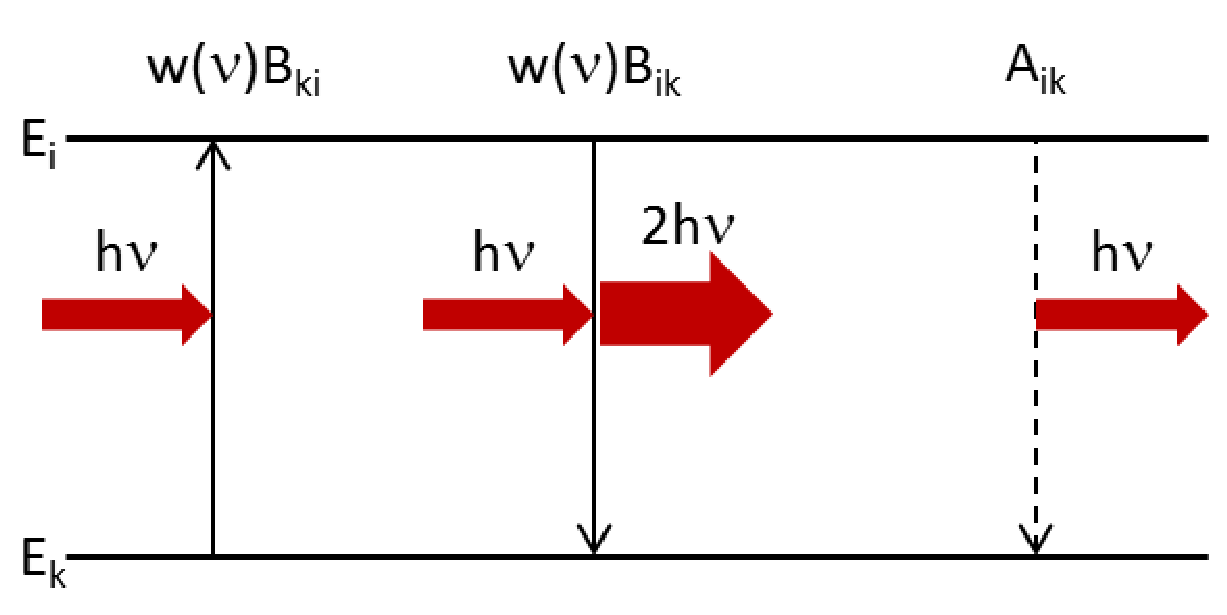
\includegraphics[width=10cm]{gfx/einstein_koeffizienten}
	}
	\caption[Einsteinkoeffizienten]{Zwei Energieniveaus eines Atoms mit Absorption,
	induzierte Emission und spontane Emission (von links nach rechts).}
	\label{fig:einstein_koeffizienten}
\end{figure}
Im thermischen Gleichgewicht folgen die Besetzungszahlen der
Boltzmann-Verteilung \cite{demtroeder:ex3}:
\begin{equation}\label{eq:boltzmann_verteilung}
	\begin{split}
		\frac{N_i}{N_k}&=\frac{g_i}{g_k}\mathrm{e}^{-\frac{(E_i-E_k)}{k_BT}}\\[0.2cm]
		&=\frac{g_i}{g_k}\mathrm{e}^{-\frac{h\nu}{k_BT}}\,.
	\end{split}	
\end{equation}
$g_i$ und $g_k$ sind die Entartungsgrade ($2J+1$) der jeweiligen Niveaus und
sind damit eine statistische Gewichtung dieser.
Kombiniert man \eqref{eq:raten_gleichung} und \eqref{eq:boltzmann_verteilung}
und löst nach $w(\nu)$ auf, findet man
\begin{equation}\label{eq:spektrale_energiedichte_1}
	w(\nu)=\frac{\nicefrac{A_{ik}}{B_{ik}}}{\left(\nicefrac{g_i}{g_k}\right)\left(\nicefrac{B_{ik}}{B_{ki}}\right)\left(\mathrm{e}^\frac{h\nu}{k_BT}-1\right)}\,.
\end{equation}
Führt man einen Koeffizientenvergleich mit der spektralen
Energiedichte eines thermischen Strahlungsfeldes \cite{demtroeder:ex3}
\begin{equation}\label{eq:spektrale_energiedichte_2}
	w(\nu)=\frac{8\pi h\nu^3}{c^3}\frac{1}{\mathrm{e}^\frac{h\nu}{k_BT}-1}
\end{equation}
durch, findet man folgende Beziehungen der Einsteinkoeffizienten:
\begin{subequations}\label{eq:einsteinkoeff_relationen}
	\begin{equation}\label{eq:einsteinkoeff_relationen_1}
		B_{ik}=\frac{g_k}{g_i}B_{ki}
	\end{equation}
	\begin{equation}\label{eq:einsteinkoeff_relationen_2}
		A_{ik}=\frac{8\pi h\nu^3}{c^3}B_{ik}\,.
	\end{equation}
\end{subequations}
%TODO: im therm. Feld ist ind. Emission viel geringer als spont.
% Emission -> kein Laser im therm. Feld
\par
Im Folgenden sollen die Einsteinkoeffizienten berechnet werden.
Zur Berechnung des Koeffizienten der spontanen Emissionswahrscheinlichkeit
betrachtet man das Atom als Hertzschen Dipol, der radial isotrop abstrahlt. Die
zeitlich mittlere abgestrahlte Leistung von $N_i$ Atomen
\cite{demtroeder:ex3} ist
\begin{equation}\label{eq:abgestrahlte_leistung_01}
	\mean{P}_t = \frac{1}{3}N_i\frac{\omega_{ik}^4}{\pi\epsilon_0
	c^3}\abs{\OPv{d}_{ik}}^2
\end{equation}
mit dem bereits erwähnten Dipolmatrixelement
$\OPv{d}_{ik}=e\bra{\Psi_i}\OPv{r}\ket{\Psi_k}$. Definiert man den
Einsteinkoeffizienten der spontanen Emission $A_{ik}$ als Wahrscheinlichkeit pro
Sekunde, dass ein Atom spontan von $\ket{\Psi_i}$ in $\ket{\Psi_k}$ übergeht,
ist Gl. \eqref{eq:abgestrahlte_leistung_01} identisch mit
\begin{equation}\label{eq:abgestrahlte_leistung_02}
	\mean{P}_t=N_iA_{ik}h\nu_{ik}\,.
\end{equation}
Daraus folgt
\begin{equation}\label{eq:einstein_koeff_A}
	A_{ik}=\frac{2}{3}\frac{\omega_{ik}^3}{\epsilon_0c^3h}\abs{\OPv{d}_{ik}}^2\,.
\end{equation}
Um die Einsteinkoeffizienten für die Absorption und induzierte Emission
zu berechnen, setzt man mit der Absorptionswahrscheinlichkeit pro Sekunde an
(FGR \eqref{eq:uebergangs_rate_total}):
\begin{equation}\label{eq:w_ki_01}
	W_{k\to i}
	= \frac{2\pi}{\hbar}\rho(E_k)\abs{\bra{\Psi_i}\OPH'\ket{\Psi_k}}^2
\end{equation}
Die Energieniveaudichte lässt sich schreiben als
$\rho(E)=\pfrac{n}{E}=\frac{1}{h}\pfrac{n}{\nu}$.
Das zeitliche Mittel der spektralen Energiedichte des elektromagnetischen Feldes
ist $\mean{w(\nu)}_t=\pfrac{n}{\nu}\frac{1}{2}\epsilon_0 E^2_0$. Damit lässt
sich die Energieniveaudichte in Relation zur spektralen Energiedichte schreiben:
\begin{equation}\label{eq:energieniveaudichte_spektrale_energiedichte}
	\rho(E)=\frac{2\mean{w(\nu)}_t}{\epsilon_0 E_0^2h}\,.
\end{equation}
Setzt man Gl. \eqref{eq:energieniveaudichte_spektrale_energiedichte} in
Gl. \eqref{eq:w_ki_01} ein und schreibt das Matrixelement
zu $\bra{\Psi_i}\OPH'\ket{\Psi_k} =
\frac{1}{2}E_0\vec{\epsilon}\cdot\OPv{d}_{ki}$ um, erhält
man unter der Annahme eines isotropen Strahlungsfeldes
($\mean{\abs{\vec{\epsilon}\cdot\vr}^2} = \frac{1}{3}\abs{\vr}^2$)
\begin{equation}\label{eq:w_ki_02}
	W_{ki}
	= \frac{2\pi^2}{3h^2\epsilon_0}\abs{\OPv{d}_{ki}}^2\mean{w(\nu)}_t\,.
\end{equation}
Ein Vergleich mit Gl. \eqref{eq:einsteinkoeff_wkten_ik} liefert
\begin{equation}\label{eq:einstein_koeff_B}
	B_{ki} = \frac{2\pi^2}{3h^2\epsilon_0}\abs{\OPv{d}_{ki}}^2\,.
\end{equation}
Das Ergebnis ist konsistent mit den in Gl.
\eqref{eq:einsteinkoeff_relationen} beschriebenen Relationen der
Einsteinkoeffizienten.

\subsection{Auswahlregeln}\label{subsec:auswahlregeln}
Damit ein Übergang im Rahmen der Dipolnäherung \textit{erlaubt} ist, darf das
Dipolmatrixelement nicht verschwinden:
\begin{equation}\label{eq:dipolmatrixelement}
	e\bra{\Psi_i}\OPv{r}\ket{\Psi_k}\neq0
\end{equation}
\textit{Verbotene} Übergänge können allerdings bei Betrachtung von
Matrixelementen höherer Ordnung sehr wohl erlaubt sein, sind jedoch sehr stark
unterdrückt. Welche Übergänge nun erlaubt und welche verboten sind, hängt von
der Konfiguration bzw. den Quantenzahlen der beiden Zustände ab:
\begin{equation}\label{eq:dipolmatrixelement_quantenzahlen}
	\bra{n_i,L_i,S_i,m_{L_i}, m_{S_i}}\OPv{r}\ket{n_k,L_k,S_k,m_{L_k}, m_{S_k}}
\end{equation}
Vorausgesetzt wird die LS-Kopplung mit
\begin{equation}\label{eq:LS-Kopplung}
	\begin{split}
		\vec{J}&=\vec{L}+\vec{S}\\
		\vec{L}&=\sum\limits_i\vec{l}_i\\
		\vec{S}&=\sum\limits_i\vec{s}_i\,.
	\end{split}
\end{equation}
Dies ist bei schweren Atomen nicht mehr gegeben. Dort dominiert die
jj-Kopplung mit
\begin{equation}\label{eq:jj-Kopplung}
	\begin{split}
		\vec{J}=\sum\limits_i\vec{j}_i\\
		\vec{j}_i=\vec{l}_i+\vec{s}_i\,.
	\end{split}
\end{equation}
\par
Da im Gesamtsystem der Drehimpuls erhalten ist, muss beim Übergang $\Delta L
=\pm1$ sein.
Bei Absorption eines Photons wird aus dem elektromagnetischen Feld ein Photon (Boson, Spin 1) mit dem Drehimpuls vom
Betrag 1 entnommen, was durch die Drehimpulsänderung des Atoms wieder
kompensiert werden muss. Analog verhält es sich bei der Emission. $\Delta L =\pm1$ kann auch mit
der erforderlichen unterschiedlichen Parität der Zustände begründet werden
($\OPP\ket{\psi}=(-1)^L\ket{\psi}$). Der Ortsoperator hat ungerade Parität.
Insgesamt muss sich bei der Berechnung des Matrixelements eine gerade Funktion
ergeben, damit dieses von 0 verschieden ist. Dies ist nur mit unterschiedlicher
Parität beider Zustände möglich $(-1)^{L_i}\neq(-1)^{L_k}$, was für ungerade
$\Delta L$ gilt. Die Begrenzung auf $\Delta L=\pm1$ ist durch den Spin 1 des
Photons begründet. Die Änderung der Projektion des Drehimpulses auf die
Quantisierungsachse ist mit der Polarisation des Photons verknüpft. Bei der
Absorption von zirkular polarisiertem Licht, das sich senkrecht zur
Quantisierungsachse ausbreitet, ist der Photonen-Drehimpuls +1 für
$\sigma^+$-Polarisation und -1 für $\sigma^-$-Polarisation. Linear polarisiertes
Licht ist eine Kombination aus $\sigma^+$- und $\sigma^-$-polarisiertem Licht.
Die Projektion des Drehimpulses ändert sich in diesem Fall nicht, es gilt also
$\Delta m_L = 0, \pm1$. Die Spinwellenfunktion wird bei Dipolübergängen nicht
beeinflusst, somit gilt $\Delta S=0$. Weiterhin gilt für $\vJ=\vL+\vS$ die
Änderung $\Delta J=0,\pm1$. $\Delta J=0$ rührt daher, dass die Änderung $\Delta
L=\pm1$ durch die entgegengesetzte Änderung $\Delta m_S=\mp1$ kompensiert
werden kann, was allerdings für $J=0\leftrightarrow0$ nicht möglich ist. Für die
Kopplung an den Kernspin gilt analoge Überlegung: $\Delta F = 0, \pm1$ außer
$F=0\leftrightarrow0$. In Tab. \ref{tab:auswahlregeln} sind alle Auswahlregeln
noch einmal aufgelistet.

\begin{table}
	%Summe der Breiten muss 0.91 mal \textwidth sein.
	\begin{tabular}{p{0.17\textwidth}p{0.36\textwidth}p{0.38\textwidth}}
		\toprule
		Regel & Ursache & Einschränkungen \\
		\midrule[1px]
		\hline
		$\Delta L = \pm1$ & Parität / Gesamtdrehimpulserhaltung & in LS-Kopplung \\
		$\Delta m_L = 0, \pm1$ & Polarisation / Drehimpuls des Photons & \\
		$\Delta S = 0$ & em. Feld koppelt nicht an Spin & gilt nicht mehr für
		schwere Atome mit jj-Kopplung \\
		$\Delta m_S = 0, \pm1$ & Spinorientierung & \\
		$\Delta J = 0, \pm1$ & Spin-Drehimpuls-Kombinationen & mit Ausnahme von
		$J=0\leftrightarrow0$
		\\
		$\Delta F = 0, \pm1$ & Kernspin-J-Kombinationen & mit Ausnahme von
		$F=0\leftrightarrow0$
		\\
		\bottomrule[1px]
	\end{tabular}
	\caption[Auswahlregeln]{Auswahlregeln, deren Ursache und Einschränkungen.}
	\label{tab:auswahlregeln}
\end{table}



\subsection{Linienprofil}\label{sec:linienprofil}
Bisher wurde noch keine Aussage über die spektralen Eigenschaften eines
Übergangs gemacht. Diese ist aber für die Laserspektroskopie von essenzieller
Bedeutung, da sie viele Informationen über die untersuchten Atome wie z.B. die
Lebensdauern der Niveaus, Sättigungsleistungen der Laser für die Übergänge oder
die Geschwindigkeitsverteilung der Atome enthalten. Auch erfährt man durch die
Kenntnis der Linienbreite, wie hoch sich bestimmte Übergänge prinzipiell
auflösen lassen und welche Lasereigenschaften dafür benötigt werden. Die
Lasereigenschaften bzw. das Laserverhalten sind ein wesentlicher Bestandteil
dieser Arbeit (siehe spätere Abschnitte \ref{sec:diodenlaser},
\ref{sec:lasersystem}, \ref{sec:stabilitaet_der_laser}). Übergänge (hier Linien genannt) sind nicht beliebig scharf, sondern
haben eine Breite, die verschiedene Ursachen hat
\cite{demtroeder:laserspektroskopie}. Die spektrale Linienbreite ist durch das Frequenzintervall $\delta\omega=\omega_2-\omega_1$ zwischen den beiden
Frequenzen, bei denen die Absorptions- bzw. Emissionsintensitäten auf die Hälfte
ihres Maximums abgesunken sind, definiert (volle Halbwertsbreite, engl.:
FWHM).

\subsubsection{Natürliche
Linienbreite}\label{subsubsec:natuerliche_linienbreite}
Die natürliche Linienbreite ist eine unvermeidliche, natürliche Gegebenheit.
Diese beruht darauf, dass man ein Atom (in klassischer Sichtweise) als
einen harmonischen, gedämpften Oszillator ansehen kann, dessen Frequenzspektrum
nicht diskret ist. Die Lösung der Bewegungsgleichung eines klassischen
Oszillators
\begin{equation}\label{eq:klassischer_oszillator_bewegungsgleichung}
	\ddot x+\gamma\dot x+\omega_0^2x=0
\end{equation}
ist
\begin{equation}\label{eq:klassischer_oszillator_loesung}
	x(t)=x_0\mathrm{e}^{-\nicefrac{\gamma t}{2}}\left[\cos(\omega
	t)+\frac{\gamma}{2\omega}\sin{(\omega t)}\right]\quad
	\text{mit}\quad \omega=\sqrt{\omega_0^2-\frac{\gamma^2}{4}}\,.
\end{equation}
Um das Frequenzspektrum zu erhalten, führt man eine Fouriertransformation durch
($x(t)\to A(\omega)$). Unter Berücksichtigung, dass man sich in nahresonanter
Umgebung befindet ($(\omega-\omega_0)^2\ll\omega_0^2$), folgt die auf die
Gesamtintensität $I_0$ normierte spektrale Intensitätsverteilung als sog.
\textit{Lorentz-Profil}
\begin{equation}\label{eq:lorentz-profil}
	\begin{split}
		I(\omega) &=A(\omega)A^*(\omega)\\
		&=
		I_0\frac{\nicefrac{\gamma}{2\pi}}{(\omega-\omega_0)^2+(\nicefrac{\gamma}{2})^2}\,.
	\end{split}
\end{equation}
Hierbei ist $\delta\omega_n=\gamma$ die natürliche Linienbreite. Weiterhin lässt
sich hier auch ein Zusammenhang zwischen der Linienbreite und der Lebensdauer
eines Zustandes herleiten. Multipliziert man die Bewegungsgleichung
\eqref{eq:klassischer_oszillator_bewegungsgleichung} mit $m\dot x$ und führt
eine Zeitableitung durch, findet man
\begin{equation}\label{eq:klassischer_oszillator_leistung_01}
	\fracd{}{t}\left[\frac{m}{2}\dot
	x^2+\frac{m}{2}\omega_0^2x^2\right]=-\gamma m\dot x^2=\fracd{W}{t}=P(t)\,,
\end{equation}
wobei $W$ die Gesamtenergie und $P(t)$ die momentan abgestrahlte Leistung des
Atoms ist. Nach Einsetzen von \eqref{eq:klassischer_oszillator_loesung} in
\eqref{eq:klassischer_oszillator_leistung_01} und zeitlicher Mittlung findet
man
\begin{equation}\label{eq:klassischer_oszillator_leistung_02}
	\mean{P(t)}_t=-\frac{1}{2}\gamma mx_0^2\omega_0^2\mathrm{e}^{-\gamma
	t}\,.
\end{equation}
Dies bedeutet, dass die Leistungsabnahme nach $\tau=\nicefrac{1}{\gamma}$ auf
$\nicefrac{1}{\mathrm{e}}$ des Anfangswertes abgefallen ist. Folglich ist die
Linienbreite $\delta\omega_i=\nicefrac{1}{\tau_i}$ eines spontanen Zerfalls von
einem Niveau $E_i$ in den Grundzustand von der Lebensdauer $\tau_i$ des
Zustands $\ket{\Psi_i}$ abhängig.
Zu diesem Ergebnis kommt man auch über die Heisenbergsche Unschärferelation bei scharf bestimmtem $\tau$:
\begin{equation}\label{eq:unschaerferelation}
	\begin{split}
		\Delta E\cdot\Delta t &\geq2\pi\hbar\\
		&\Leftrightarrow\\
		\hbar\,\delta\omega\cdot2\pi\tau &\geq2\pi\hbar\\
		&\Leftrightarrow\\
		\delta\omega &\geq\frac{1}{\tau}\,.
	\end{split}
\end{equation}
Die Linienbreite eines Übergangs zwischen
zwei angeregten Niveaus $E_i$ und $E_k$ ergibt sich aus den Lebensdauer beider Niveaus mit
\begin{equation}\label{eq:natuerliche_linienbreite_lebensdauern}
	\delta\omega_{i\leftrightarrow
	k}=\frac{1}{\tau_i}+\frac{1}{\tau_k}\,.
\end{equation}

\subsubsection{Sättigungsverbreiterung}\label{subsubsec:saettigungsverbreiterung}
Die Sättigungsverbreiterung der Linie tritt erst durch Einstrahlen von
Laserlicht in Erscheinung. Sie ist gerade bei hohen Laserleistungen von
Bedeutung. Sehr elegant lässt sich die Sättigungsverbreiterung über den
\textit{Dichtematrix-Formalismus} herleiten.\par
Im Experiment sind die Atome aufgrund der spontanen Emission statistisch
verteilt und somit dephasiert. Es liegt kein \textit{reiner Zustand}\footnote{Reiner Zustand: Es
besteht eine kohärente Überlagerung der Zustände:
$\ket{\Psi}=\frac{1}{\sqrt{2}}\left[\alpha(t)\mathrm{e}^{\mathrm{i}\phi}\keta+\beta(t)\ketb\right]$,
wobei die Phase $\phi$ immer konstant bleibt.} mehr vor, sondern ein
\textit{statistisches Gemisch}. Die Phase zwischen den Zuständen ist
für jedes Atom individuell im Intervall $[0,2\pi)$ verteilt\footnote{$[x,y)$
steht für ein halboffenes Intervall "`x bis y, exklusive y"'.}.
Somit ist eine einfache Behandlung mit der Schrödingergleichung nicht mehr
möglich. Der Dichtematrix-Formalismus berücksichtigt diese Tatsache allerdings. Dazu betrachtet man die Dichtematrix
\begin{equation}\label{eq:dichtematrix}
	\OP{\rho}
	=
	\begin{pmatrix}
		\rho_{11} & \rho_{12}\\
		\rho_{21} & \rho_{22}
	\end{pmatrix}
	=
	\begin{pmatrix}
		c_1c_1^* & c_1c_2^*\\
		c_2c_1^* & c_2c_2^*
	\end{pmatrix}\,.
\end{equation}
$\rho_{11}$ bzw. $\rho_{22}$ sind die Besetzungswahrscheinlichkeiten von
$\ket{1}$ bzw. $\ket{2}$. $\rho_{12}$ und $\rho_{21}$ sind die
Kohärenzen beider Zustände, wobei $\rho_{12}=\rho_{21}^*$ ist. $c_i$ bzw.
$c_i^*$ sind wiederum die Zeitentwicklungskoeffizienten der Zustände $\ket{i}$.
Die Bewegungsgleichungen dieser Koeffizienten erhält man aus dem
nicht-störungstheoretischen Ansatz eines 2-Niveau-Systems, welcher wie folgt
aussieht:
\begin{subequations}\label{eq:2-niveau-system_ansatz}
	\begin{equation}\label{eq:2-niveau-system_ansatz_hamilton}
		\begin{split}
			\OPH &=\OPH_0-\vd\cdot\vE(t)\\
			\text{mit}\quad
			\vE(t) &=\vec{\epsilon}E_0\cos{(\omega t)}\\
			\text{und}\quad
			\OPH_0 &=\hbar\omega_1\ket{1}\bra{1}+\hbar\omega_2\ket{2}\bra{2}
		\end{split}
	\end{equation}
	\begin{equation}\label{eq2-niveau-system_ansatz_zustand}
		\ket{\Psi}=c_1(t)\mathrm{e}^{-\mathrm{i}\omega_1
		t}\ket{1}+c_2(t)\mathrm{e}^{-\mathrm{i}\omega_2 t}\ket{2}\,.
	\end{equation}	
\end{subequations}
Gleichung \ref{eq:2-niveau-system_ansatz_hamilton} beschreibt den
Hamilton-Operator, Gleichung \ref{eq2-niveau-system_ansatz_zustand} beschreibt
den Zustand eines 2-Niveau-Systems. Nach Einsetzen in die Schrödingergleichung
und etwas längerer Rechnung findet man
\begin{subequations}\label{eq:2-niveau-system_koeffizienten}
	\begin{equation}\label{eq:2-niveau-system_c1}
		\dot c_1(t)=\frac{\mathrm{i}\Omega_0}{2}\mathrm{e}^{\mathrm{i}\delta t}c_2(t)
	\end{equation}
	\begin{equation}\label{eq:2-niveau-system_c2}
		\dot c_2(t)=\frac{\mathrm{i}\Omega_0}{2}\mathrm{e}^{\mathrm{i}\delta
		t}c_1(t)\,,
	\end{equation}	
\end{subequations}
wobei $\delta$ die Verstimmungsfrequenz zwischen Lichtfeld und atomarem Übergang
ist ($\delta=\omega-\omega_{21}$\,, $\omega_{21}=\omega_2-\omega_1$).
$\Omega_0=\nicefrac{dE_0}{\hbar}$ ist die sog. \textit{Rabifrequenz}\footnote{Die Rabifrequenz
ist die Frequenz mit der das 2-Niveau-System zwischen Grundzustand und
angeregtem Zustand oszilliert, sofern kontinuierlich resonantes Licht
eingestrahlt wird.}, welche aber im Folgenden nicht von Interesse ist.
Betrachtet man die Zeitentwicklung der Dichtematrixelemente
\begin{equation}\label{eq:dichtematrix_zeitentwicklung}
	\fracd{}{t}\OP{\rho}
	=
	\begin{pmatrix}
		\dot c_1c_1^*+c_1\dot c_1^* & \dot c_1c_2^*+c_1\dot c_2^*\\
		\dot c_2c_1^*+c_2\dot c_1^* & \dot c_2c_2^*+c_2\dot c_2^*
	\end{pmatrix}
\end{equation}
und setzt nun Gln. \ref{eq:2-niveau-system_koeffizienten} in Gl.
\ref{eq:dichtematrix_zeitentwicklung} ein, ergeben sich die sog.
\textit{optischen Bloch-Gleichungen} (OBE's):
\begin{subequations}\label{eq:blochgleichungen_01}
	\begin{equation}\label{eq:blochgleichungen_11}
		\fracd{}{t}\rho_{11}=\gamma\rho_{22}+\mathrm{i}\frac{\Omega_0}{2}(\tilde\rho_{21}-\tilde\rho_{12})
	\end{equation}
	\begin{equation}\label{eq:blochgleichungen_22}
		\fracd{}{t}\rho_{22}=-\gamma\rho_{22}+\mathrm{i}\frac{\Omega_0}{2}(\tilde\rho_{12}-\tilde\rho_{21})
	\end{equation}
	\begin{equation}\label{eq:blochgleichungen_12}
		\fracd{}{t}\tilde\rho_{12}=-\left(\frac{\gamma}{2}+\mathrm{i}\delta\right)\tilde\rho_{12}+\mathrm{i}\frac{\Omega_0}{2}(\rho_{22}-\rho_{11})
	\end{equation}
	\begin{equation}\label{eq:blochgleichungen_21}
		\fracd{}{t}\tilde\rho_{21}=-\left(\frac{\gamma}{2}+\mathrm{i}\delta\right)\tilde\rho_{21}+\mathrm{i}\frac{\Omega_0}{2}(\rho_{11}-\rho_{22})\,.
	\end{equation}	
\end{subequations}
Hierbei wurde direkt schon die spontane Emissionsrate $\gamma$ von Niveau
$\ket{2}$ zu Niveau $\ket{1}$ eingepflegt.
$\tilde\rho_{12}=\mathrm{e}^{-\mathrm{i}\delta t}\rho_{12}$ und $\tilde\rho_{21}=\mathrm{e}^{\mathrm{i}\delta
t}\rho_{21}$ bedeutet, dass $\rho_{ij}$ ($i\neq j$) in ein rotierendes
Bezugssystem mit Frequenz $\delta$ transformiert worden sind. Da für die
Kohärenzen $\rho_{12}=\rho_{21}^*$ gilt, reduzieren sich die OBE's zu zwei
unabhängigen Gleichungen
\begin{subequations}\label{eq:blochgleichungen_02}
	\begin{equation}\label{eq:blochgleichungen_21_1}
		\fracd{}{t}\tilde\rho_{21}=-\left(\frac{\gamma}{2}-\mathrm{i}\delta\right)\tilde\rho_{21}-\frac{\mathrm{i}w\Omega_0}{2}
	\end{equation}
	\begin{equation}\label{eq:blochgleichungen_w}
		\fracd{}{t}w=-\gamma(w+1)-\mathrm{i}\Omega_0(\tilde\rho_{21}-\tilde\rho_{12})
	\end{equation}	
\end{subequations}
mit der \textit{Besetzungsinversion} $w=\rho_{22}-\rho_{11}$. Sie gibt an, wie
stark die Besetzung im Zustand $\ket{2}$ gegenüber der im Zustand $\ket{1}$ ist.
Für lange Zeiten stellt sich (nach ausgemittelten Rabioszillationen) ein
Gleichgewicht ein, wobei beide Niveaus bestenfalls gleich stark besetzt sind. Dies ist mit der Bedingung gegeben,
dass sich die Besetzungsinversion und die Kohärenzen nicht mehr ändern:
\begin{equation}\label{eq:blochgleichungen_gleichgewicht}
	\begin{split}
		\fracd{}{t}\tilde\rho_{21} &=\fracd{}{t}w=0\\
		&\Leftrightarrow\\
		w &=-\frac{1}{1+S}\\
		\text{und}\quad
		\tilde\rho{21}
		&=\frac{\mathrm{i}\Omega_0}{2(\nicefrac{\gamma}{2}-\mathrm{i}\delta)(1+S)}\,.
	\end{split}
\end{equation}
Hier wurde der \textit{Sättigungsparameter}
\begin{equation}\label{eq:saettigungsparameter}
	S=\frac{S_0}{1+\nicefrac{4\delta^2}{\gamma^2}}
\end{equation}
mit dem \textit{resonanten Sättigungsparameter}
\begin{equation}\label{eq:saettigungsparameter_0}
	S_0=\frac{2\Omega_0^2}{\gamma^2}
\end{equation}
eingeführt. Für die Population des angeregten Zustandes erhält man mit
$\rho_{11}+\rho_{22}=1$
\begin{equation}\label{eq:besetzung_22}
	\rho_{22}=\frac{1}{2}(1+w)=\frac{S}{2(1+S)}=\frac{\nicefrac{S_0}{2}}{1+S_0+\nicefrac{4\delta^2}{\gamma^2}}\,.
\end{equation}
Nebenbei kann man hierbei die sehr wichtige Tatsache, dass die Population des
angeregten Zustandes \textit{niemals größer als $50\,$\%} sein kann, ablesen:
\begin{equation}\label{eq:besetzung_22_kleiner-gleich_50}
	\lim_{S\to\infty}\rho_{22}=\frac{1}{2}\,.
\end{equation}
Weiterhin ergibt sich aus Gl. \eqref{eq:besetzung_22} die Photonenstreurate
\begin{equation}\label{eq:photonenstreurate_01}
	\Gamma_{ph}=\gamma\rho_{22}=\frac{\gamma}{2}\frac{S_0}{1+S_0+\nicefrac{4\delta^2}{\gamma^2}}\,,
\end{equation}
die im Gleichgewicht gleich der Absorptionsrate ist.
Nach einer Umformung
\begin{equation}\label{eq:photonenstreurate_02}
	\Gamma_{ph}=\left(\frac{S_0}{1+S_0}\right)\left(\frac{\nicefrac{\gamma}{2}}{1+\nicefrac{4\delta^2}{\gamma'^2}}\right)
	\quad\text{mit}\quad
	\gamma'=\gamma\sqrt{1+S_0}
\end{equation}
sieht man bei Vergleich mit \eqref{eq:lorentz-profil}, dass sich die
Linienbreite um den Faktor $\sqrt{1+S_0}$ vergrößert hat. Diese Verbreiterung
nennt man Sättigungsverbreiterung. Wichtig ist auch die Abhängigkeit von $S_0$
von den physikalischen Größen des Übergangs und des verwendeten Lasers.
Kombiniert man Gl. \eqref{eq:saettigungsparameter_0} mit
$\Omega_0=\nicefrac{dE_0}{\hbar}$, $I=\nicefrac{1}{2}c\epsilon_0E_0^2$ und der
spontanen Zerfallsrate \eqref{eq:abgestrahlte_leistung_02} erhält man
\begin{equation}\label{eq:saettigungsparameter_physikalische_groessen}
		S_0=\frac{I}{I_{sat}}
		\quad\text{mit}\quad
		I_{sat}=\frac{\pi hc}{3\lambda^3\tau}\,.
\end{equation}
Mit \eqref{eq:photonenstreurate_02} bedeutet das, dass die Linienbreite eines
Übergangs mit der Wurzel der Laserintensität $I$ wächst. Des Weiteren
ist zu erkennen, dass die Erhöhung der Laserleistung irgendwann nicht mehr
von Belang ist, da sich der Vorfaktor $\nicefrac{S_0}{\left(1+S_0\right)}$ in
\eqref{eq:photonenstreurate_02} asymptotisch gegen 1 nähert.
Sättigungsleistungen $I_{sat}$ in den optischen Übergängen der später in dieser
Arbeit behandelten Ionisations-Schemata bewegen sich im Bereich von wenigen
mW bei den ersten beiden Anregungsschritten bis hin zu einigen
$100\,$mW beim autoionisierenden Schritt.
%TODO: !!Bild: Sättigungsverbreiterte Linie

\subsubsection{Dopplerverbreiterung}\label{subsubsec:doppler-verbreiterung}
In der Regel bewegen sich die zu untersuchenden Atome relativ zum Wellenvektor
$\vk$ des Laserlichts. Für ein Atom, das sich auf das Laserlicht zubewegt,
verschiebt sich aufgrund des Dopplereffekts die Frequenz ins blaue. Analog
verschiebt sich die Frequenz für das Atom ins rote, wenn es sich in Richtung der Photonen bewegt. Durch Einstrahlen von entsprechend entgegengesetzt zur
Ruhefrequenz $\omega_0$ verstimmtem Licht mit der Frequenz
\begin{equation}\label{eq:doppler}
	\omega=\omega_0+k_zv_z=\omega_0\left(1+\frac{v_z}{c}\right)
\end{equation}
kann dies kompensiert und die Resonanz wieder getroffen werden. Statistisch sind
die Atome im Experiment allerdings geschwindigkeitsverteilt
\cite{demtroeder:laserspektroskopie} mit
\begin{equation}\label{eq:boltzmann-verteilung_v}
	n_i(v_z)\dd{v_z}=\frac{N_i}{v_w\sqrt{\pi}}\mathrm{e}^{-\left(\frac{v_z}{v_w}\right)^2}\dd{v_z}\,,
\end{equation}
wobei $v_w=\sqrt{\nicefrac{2k_BT}{m}}$ die wahrscheinlichste Geschwindigkeit und
$N_i$ die Anzahl der Atome im Zustand $\ket{\Psi_i}$ ist. Für die Gauß-förmige
Frequenzverteilung folgt dann
\begin{equation}\label{eq:boltzmann-verteilung_omega}
	n_i(\omega)\dd\omega=\frac{cN_i}{v_w}\omega_0\sqrt{\pi}\mathrm{e}^{-\left[\frac{c(\omega-\omega_0)}{\omega_0v_w}^2\right]}\dd\omega\,.
\end{equation}
Das Linienprofil ist proportional zu $n_i(\omega)$ und somit auch Gauß-verteilt.
Für die Halbwertsbreite der Dopller-verbreiterten Linie folgt somit  
\begin{equation}\label{eq:doppler-breite}
	\delta\omega_D=\frac{\omega_0}{c}\sqrt{\frac{8k_BT\mathrm{ln}2}{m}}\,.
\end{equation}
Die Dopplerverbreiterung nimmt also linear mit der Frequenz des eingestrahlten
Lichts zu und wird bei hohen Temperaturen und leichten Atomen sehr groß. Sie
kann die natürliche Linienbreite um gut zwei Größenordnungen übertreffen. Um die
Dopplerverbreiterung möglichst gering zu halten, wird im Experiment das
Laserlicht transversal zur Austrittsrichtung der Atome aus dem Ofen
eingestrahlt. Außerdem wird das Licht für die einzelnen Anregungsschritte in
zueinander kollinearer Richtung eingestrahlt, damit die Summenfrequenz aller
drei Photonen auf nahezu alle Dopplerklassen erweitert wird. Wie sich in Absch.
\ref{subsec:mehrfach_resonante_anregung} zeigen wird, ist die
Dreiphotonensumme ausschlaggebend für die Ionisationseffizienz.\par
Um das gesamte Linienprofil des Atoms zu erhalten, muss das gaußförmige
Dopller-Profil mit dem sättigungsverbreiterten Lorentzprofil gefaltet werden:
\begin{equation}\label{eq:voigt_doppler}
	V_{Atom}(\omega)=\int{L_{nat+sat}(\omega-\omega')G_{Doppler}(\omega')\dd\omega'}\,.
\end{equation}
Die Faltung eines Gauß-Profils mit einem Lorentz-Profil ergibt ein sog.
\textit{Voigt-Profil}.

\subsubsection{Stoßverbreiterung}\label{subsubsec:stossverbreiterung}
Ein im Rahmen dieser Arbeit zwar zu vernachlässigender aber erwähnenswerter
Faktor für das Linienprofil ist die Stoßverbreiterung, auch
Druckverbreiterung genannt. Dabei wird die Änderung der Linienbreite durch die
Wechselwirkung zweier Atome betrachtet. Kommen sich zwei Atome hinreichend nahe,
verschieben sich die Energieniveaus und somit die Übergangsfrequenz geringfügig. Es kann zu
elastischen und inelastischen Stößen kommen. Im Bild des klassischen Oszillators
ändert sich beim inelastischen Stoß die Amplitude, was analog zur natürlichen
Dämpfung als weitere Dämpfung interpretiert werden kann. Die Linienbreite wird
somit größer. Elastische Stöße ändern neben der kurzzeitigen Frequenzverstimmung
zusätzlich die Phase des Oszillators. Somit kommt es bei elastischen Stößen
zusätzlich zu einer Linienverschiebung. Da hier allerdings mit
sehr niedrigen Drücken (zwischen $10^{-6}$ und $10^{-8}\,$mbar) gearbeitet wird,
kann dieser Effekt vernachlässigt werden.

\subsubsection{Gesamtes Linienprofil}\label{subsubsec:ges-linienprofil}
Nicht nur die atomaren Übergänge der Atome, sondern ebenso das Linienprofil
des Lasers selbst tragen zum gesamten Linienprofil bei. Um das effektive
Linienprofil zu erhalten, muss das Profil des Lasers mit dem der atomaren
Übergänge aus Gl. \eqref{eq:voigt_doppler} gefaltet werden:
\begin{equation}\label{eq:voigt}
	\begin{split}
		V_{ges}(\omega)
		&=\int{G_{Laser}(\omega-\omega')V_{Atom}(\omega')\dd\omega'}\\
		&=\int{G_{Laser}(\omega-\omega')\left(\int{L_{nat+sat}(\omega'-\omega'')G_{Doppler}(\omega'')\dd\omega''}\right)\dd\omega'}\,.
	\end{split}
\end{equation}
Das Profil des Lasers ist ein Gauß-Profil. Das Profil eines atomaren Übergangs
im Experiment ist im Wesentlichen ein Voigt-Profil (Faltung aus Lorentz- und
Gauß-Profil), wie sich oben gezeigt hat. Da in der Algebra der Faltung
Kommutativität und Assoziativität gelten und die Faltung zweier Gauß-Profile
wieder ein Gauß-Profil ergibt, erhält man insgesamt ein Voigt-Profil.
%TODO: !Bild Voigt-Profil /Peudo-Voigt-Profil

\subsubsection{Homogene und inhomogene
Linienverbreiterung}\label{subsubsec:homogene_inhomogene_verbreiterung}
Man muss bei den einzelnen Linienverbreiterungseffekten zwischen einer
\textit{homogenen} und einer \textit{inhomogenen Linienverbreiterung}
unterscheiden. Ist eine Linienverbreiterung für alle Atome identisch vorhanden,
so nennt man sie homogen. Dies ist bei der natürlichen Linienbreite, der
Sättigungsverbreiterung und der inelastischen Stoßverbreiterung der Fall. Ein
Beispiel für die inhomogene Linienverbreiterung ist die Dopplerverbreiterung.
Hier ist die Wahrscheinlichkeit eines Übergangs abhängig von der parallelen
Geschwindigkeitskomponente der Atome zum eingestrahlten Licht. Bei elastischen
Stößen kommt es außerdem zur Umverteilung der Doppler-Klassen. Ist die Stoßzeit
zwischen zwei Stößen größer als die Licht-Atom-Wechselwirkungszeit, tragen die
Stöße nicht zur homogenen Linienverbreiterung bei. Andernfalls ist die
Umverteilung der Doppler-Klassen gleichmäßig, was zur homogenen Verbreiterung
führt. 

\section{Resonanzionisationsspektroskopie}\label{sec:ris}
Die Resonanzionisationsspektroskopie, kurz RIS, ist eine weit verbreitete
Methode, Atome spektroskopisch zu untersuchen. Dabei werden die erzeugten Atome
über mehrstufige Anregung (Abschn. \ref{subsec:mehrfach_resonante_anregung})
ionisiert (Abschn. \ref{subsec:ionisation}) und anschließend mittels
einer Ionenoptik zu einem Detektor geführt, wo sie nachgewiesen werden. Der
große Unterschied zu anderen laserspektroskopischen Methoden wie
etwa die Absorptions- und Fluoreszenzspektroskopie ist die Tatsache, dass
hierbei Ionen, mit einer Effizienz von nahezu $\epsilon=1$, anstatt Photonen mit
einer üblicherweise wesentlich geringeren Effizienz von $\epsilon\leq10^{-4}$
detektiert werden.\par
Zusätzlich erfolgt die Ionisation bei der RIS elementselektiv, was
bedeutet, dass über für jedes Element charakteristische Anregungsschritte
ionisiert wird.
Auch eine Isotopenselektivität ist bei der RIS insofern gegeben, dass die
atomaren Übergänge einer Isotopieverschiebung (Abschn. \ref{subsec:isotopieverschiebung})
unterliegen und so jedes Anregungsschema eines jeden Isotops individuell
ist. Die Isotopieverschiebungen der Übergänge des in diesem Projekt
untersuchten Urans sind dabei typischerweise mehrere
GHz groß. Mit gepulst betriebenen, breitbandigen
Titan-Saphir-Lasern, wie sie u.a. in der AG Larissa in Mainz verwendet werden,
ist eine gute Isotopenselektivität nicht mehr gegeben, da ihre Linienbreite
gleichermaßen bei mehreren GHz liegt. Um hochselektive RIS zu betreiben,
werden in diesem Projekt kontinuierlich betriebene und damit schmalbandige
Diodenlaser (Abschn. \ref{sec:diodenlaser}) verwendet, deren Linienbreite bei nur einigen
MHz liegt.\par
Eine Erweiterung der RIS ist die sog. Resonanzionisationsmassenspektrometrie,
kurz RIMS. Hierbei werden die Ionen vor der Detektion zusätzlich in einem
Massenspektrometer nach ihrer Masse selektiert, was eine Trennung der Isotope
garantiert. Auch werden Ionen anderer Elemente oder Moleküle mit verschiedener
Masse gegenüber dem untersuchten Isotop unterdrückt. In Kap.
\ref{kap:experimenteller_aufbau} wird im Rahmen des experimentellen Aufbaus noch
einmal auf die Massentrennung, die mithilfe eines Quadrupolmassenfilters
geschieht, eingegangen. Das Hauptaugenmerk liegt in dieser Arbeit allerdings auf der RIS
und dem dabei verwendeten Lasersystem.

\subsection{Mehrfach
resonante Anregung}\label{subsec:mehrfach_resonante_anregung}
Wie in Abschn. \ref{sec:licht-atom-wechselwirkung} schon erklärt, können Atome
durch Absorption resonant in ein höher liegendes Energieniveau gebracht werden.
Durch Kombination von aneinandergereihten Anregungsschritten kann
das Atom in einen Zustand oberhalb des \textit{Ionisationspotentials} gebracht
und somit ionisiert werden. Typischerweise werden in diesem Projekt dreistufige
Anregungsschemata verwendet, wobei der dritte Schritt das Atom einfach
positiv ionisiert. Um das Anregungsverhalten theoretisch zu beschreiben, reicht
es dabei nicht aus, mehrere Zwei-Niveau-Systeme aneinandergereiht zu betrachten,
da damit kohärente Prozesse und die dadurch gegebenen Kohärenzen zwischen den
Zuständen vernachlässigt werden. Es muss dazu ein Dichtematrixformalismus für
ein 3-Niveau-System entwickelt werden, der die Prozesse Absorption, induzierte Emission und spontane Emission für alle
Niveaus des Systems mit einbezieht. Für ein
Zwei-Niveau-System wurde dies in Abschn.
\ref{subsubsec:saettigungsverbreiterung} angedeutet. Für ein N-Niveau-System mit
$N\geq3$ verkompliziert sich die theoretische Beschreibung deutlich und wird
deshalb in dieser Arbeit nicht weiter behandelt. Es sei für die theoretische Beschreibung im Allgemeinen auf \cite{blum:density_matrix_theory} und für die
Beschreibung in Bezug auf die RIS an Calcium-Atomen auf
\cite{noertershaeuser:1999:dissertation} verwiesen. In
\cite{schumann:2005:dissertation} wurde die Ionisationseffizienz als Funktion
der Verstimmung der ersten beiden Anregungsschritte von Uran theoretisch
berechnet. Abbildung \ref{fig:2D-laserscan_theorie_schumann} zeigt diese
Abhängigkeit.
\begin{figure}[h]
	\centering
	\fbox{
		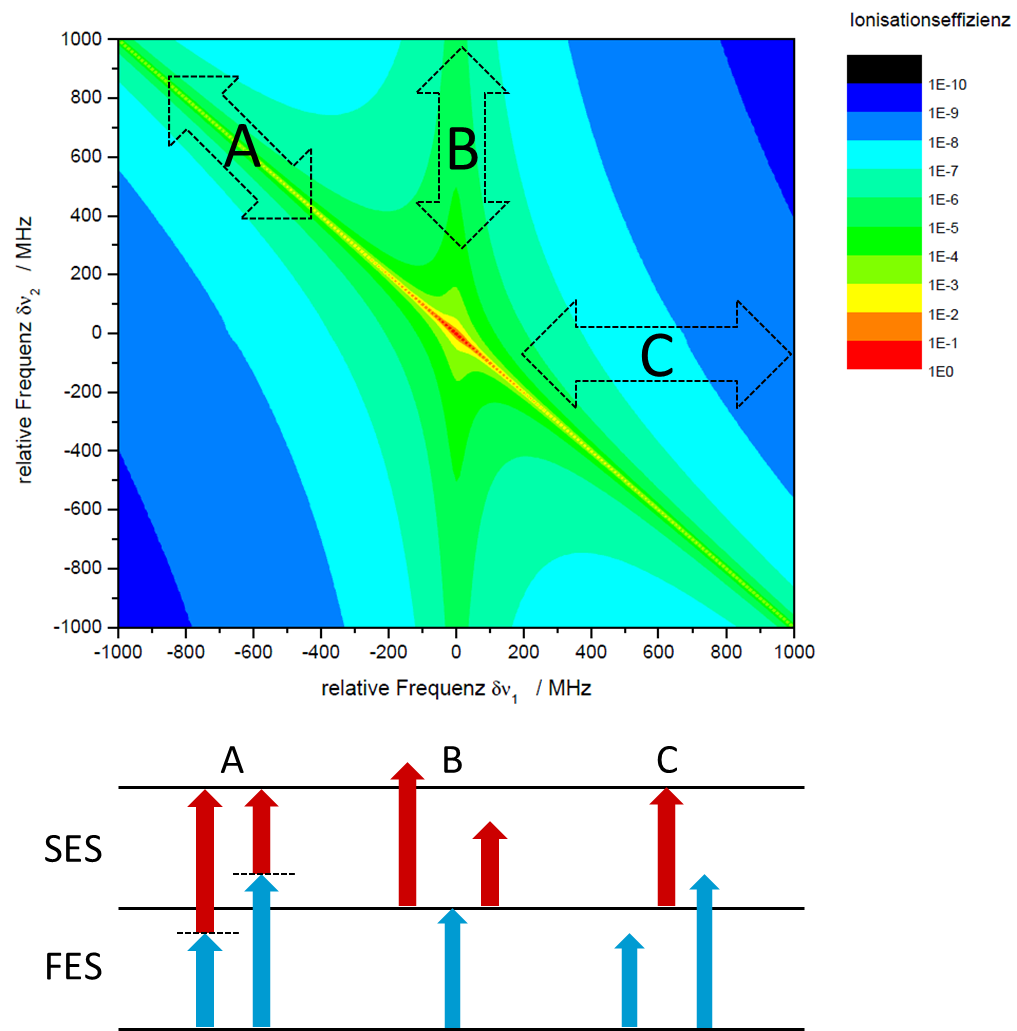
\includegraphics[width=\textwidth-1cm]{gfx/2d-laserscan_theorie_schumann.png}
	}
	\caption[2D-Laserscan]{Dopplerfreie
	Ionisationseffizienz in Abhängigkeit
	der Verstimmungen der beiden ersten
	Anregungsschritte mit den Strukturen
	der Einphoton-Resonanz (B), (C) und
	Zweiphotonen-Resonanz (A).
	Erklärungen im Text. (aus
	\cite{schumann:2005:dissertation})}
	\label{fig:2D-laserscan_theorie_schumann}
\end{figure}
Die Strukturen zeigen, dass sich kein zweidimensionales
Voigtprofil ergibt. Die diagonale Struktur A
resultiert aus der \textit{Zweiphotonen-Resonanz}. Dabei ist die Summenfrequenz
der ersten beiden Anregungsschritte gleich der Übergangsfrequenz vom
Grundzustand (GZ) zum zweiten angeregten Zustand (SES, \textit{second excited
state}).
Auch bei relativ großer Verstimmung zum SES erhält man entlang dieser Linie noch
signifikante Übergangsraten.
Die Struktur B zeigt die \textit{Einphotonen-Resonanz} bei resonantem ersten Übergang. Auch
hier ergeben sich deutlich erhöhte Raten bei großer Verstimmung des zweiten
Schrittes, aber bereits deutlich schwächer als bei der Zweiphotonen-Resonanz.
Hält man im Gegensatz dazu den zweiten Schritt in Resonanz und verstimmt den
ersten Schritt, fällt die Ionisationseffizienz sehr schnell ab (Struktur C), da
diese maßgeblich von der Population des ersten angeregten Zustandes
(FES, \textit{first excited state}) abhängt. Weitere Anregungen
bis zur Ionisation werden somit weitaus unwahrscheinlicher, als wenn die
Population erst in höheren Zuständen durch nicht-Resonanz abnimmt.

\subsection{Ionisation}\label{subsec:ionisation}
Um die Atome nach dem letzten Anregungsschritt zu ionisieren, muss
ein Niveau besetzt werden, das oberhalb des Ionisationspotentials liegt. Dies
kann durch drei verschiedene Prozesse geschehen: \textit{Feldionisation},
\textit{nicht-resonante Photoionisation} und \textit{Autoionisation}. Da die
ersten beiden Prozesse in diesem Projekt keine Anwendung finden bzw.
keinen nennenswerten Beitrag haben, seien diese nur am Rande erwähnt und es soll
speziell auf die Autoionisation detailliert eingegangen werden.

\subsubsection{Feldionisation}\label{subsubsec:feldionisation}
Durch Anlegen eines elektrischen Feldes in der Wechselwirkungsregion kann das
Ionisationspotential abgesenkt werden, wodurch gebundene Zustände oberhalb des
Ionisationspotentials zu liegen kommen und somit durch resonante Anregung in
diese Zustände eine Ionisation möglich ist. Da allerdings hierfür
vergleichsweise starke Felder nötig sind, kommt es ungünstigerweise zu
\textit{Stark-Shifts}\footnote{Der \textit{Stark-Shift} bezeichnet die
energetische Aufspaltung (Aufhebung der Entartung) atomarer oder molekularer
Zustände in Anwesenheit eines externen elektrischen Feldes (analog zum
Zeeman-Effekt bei externen magnetischen Feldern).}.
%TODO: Bild Feldionisation, nicht-resonante Ionisation

\subsubsection{nicht-resonante
Photoionisation}\label{subsubsec:nicht-resonante_photoionisation}
Neben resonanten Übergängen sind auch nicht-resonante Anregungen in das
Kontinuum möglich. Vorraussetzung hierfür ist, dass die gesamte Photonenenergie
aller Anregungsschritte inklusive der Photonenenergie des ionisierenden Schritts
größer ist als das Ionisationspotential
($\hbar\omega_1+\hbar\omega_2+\hbar\omega_3>\E_{IP}$). Da jedoch der
Wirkungsquerschnitt für solch einen Prozess gegenüber resonanten Prozessen
stark unterdrückt ist, wird hierfür sehr hohe Laserleistung
benötigt.

\subsubsection{Autoionisation}\label{subsubsec:autoionisation}
% Anders als z.B. beim Wasserstoffatom haben komplexe Atome kein flaches
% Anregungsspektrum in das \textit{Kontinuum}, welches alle Zustände, die ein
% Elektron frei vom Atom beschreiben, zusammenfasst. Es sind hingegen sog.
% \textit{autoionisierende Resonanzen} in der Form von mehreren GHz breiten Peaks
% zu beobachten. Das Zustandekommen dieser Strukturen lässt sich durch Anregung
% mehrerer Elektronen in der Hülle des Atoms erklären, wobei die Elektronen die
% Energie an ein Valenzelektron abgeben und dieses sich vom Restatom lösen kann.
% Die Gesamtenergie der Anregung muss dabei oberhalb des Ionisationspotentials
% liegen.
Für die in diesem Projekt verwendete Autoionisation muss das zu untersuchende
atomare System Anregungszustände besitzen, die oberhalb des
Ionisationspotentials liegen.
Bei komplexen Atomen wie Uran kommt es häufig vor, dass bestimmte Anregungsschritte durch die
Anregung mehrerer Elektronen charakterisiert sind.
Starke Überlappungen der Elektronen-Wellenfunktionen begünstigen den
Energieübertrag zwischen den Elektronen, wodurch ein Valenzelektron energetisch über das Ionisationspotential
gehoben werden kann und das Atom in ein Ion und ein freies Elektron zerfällt.
Dazu muss die Gesamtenergie der Anregung oberhalb des Ionisationspotentials
liegen.
Die Lebensdauer solcher Zustände kann bis zu 3-4 Größenordnungen kleiner sein
als die der Zustände unterhalb des Ionisationspotentials, wobei die spektrale
Breite gemäß der Unschärferelation entsprechend größer ist.
Sofern diese sog. \textit{autoionisierenden Resonanzen} Linienbreiten aufweisen,
die nicht wesentlich größer sind als die spektrale Breite des ionisierenden
Lasers, können die Wirkungsquerschnitte die der nichtresonanten Photoionisation
um mehrere Größenordnungen überschreiten. Unter Verwendung von
cw-Lasern\footnote{cw: "`continuous wave"', zu deutsch: "`kontinuierliche
Welle"', Bezeichnung für Dauerstrichlaser} reichen zur Autoionisation meist
Leistungen im Bereich von wenigen $100\,$mW aus.\par
Um den Prozess der Autoionisation theoretisch zu beschreiben, betrachtet man als
Endzustand eine Linearkombination aus einem diskreten Niveau und dem Kontinuum:
\begin{equation}\label{eq:uebergang_diskret_kontinuum}
	\ket{E}=a\ket{\phi}+\int b_\epsilon\ket{\epsilon}\dd\epsilon\,.
\end{equation}
Nach einem zeitunabhängigen störungstheoretischen Ansatz
\begin{equation}\label{eq:uebergang_diskret_kontinuum_hamilton}
	\OPH=\OPH_0+V
\end{equation}
mit $\OPH_0$ als ungestörten, in der Basis
$\left(\ket{\phi}\text{,}\,\ket{\epsilon}\right)$ diagonalisierten
Hamiltonoperator und der Störung $V$, findet man nach längerer Rechnung,
welche in \cite{fano:1961:PhysRev.124.1866} ausgeführt ist, den
Wirkungsquerschnitt
\begin{equation}\label{eq:fano-profil}
	\sigma(q,\Gamma,E_0,\epsilon)=\frac{\left(\nicefrac{q\Gamma}{2}+\epsilon-E_0\right)^2}{\left(\epsilon-E_0\right)^2+\left(\nicefrac{\Gamma}{2}\right)^2}
\end{equation}
der autoionisierenden Resonanz. Dabei sind $q$ der Formparameter, $\Gamma$ die
Linienbreite und $E_0$ die Energielage der Resonanz. In Abb. \ref{fig:fano} ist
der Wirkungsquerschnitt als sog. \textit{Fano-Profil} noch einmal grafisch
dargestellt.
\begin{figure}
	\centering
	\footnotesize
	% GNUPLOT: LaTeX picture with Postscript
\begingroup
  \makeatletter
  \providecommand\color[2][]{%
    \GenericError{(gnuplot) \space\space\space\@spaces}{%
      Package color not loaded in conjunction with
      terminal option `colourtext'%
    }{See the gnuplot documentation for explanation.%
    }{Either use 'blacktext' in gnuplot or load the package
      color.sty in LaTeX.}%
    \renewcommand\color[2][]{}%
  }%
  \providecommand\includegraphics[2][]{%
    \GenericError{(gnuplot) \space\space\space\@spaces}{%
      Package graphicx or graphics not loaded%
    }{See the gnuplot documentation for explanation.%
    }{The gnuplot epslatex terminal needs graphicx.sty or graphics.sty.}%
    \renewcommand\includegraphics[2][]{}%
  }%
  \providecommand\rotatebox[2]{#2}%
  \@ifundefined{ifGPcolor}{%
    \newif\ifGPcolor
    \GPcolortrue
  }{}%
  \@ifundefined{ifGPblacktext}{%
    \newif\ifGPblacktext
    \GPblacktexttrue
  }{}%
  % define a \g@addto@macro without @ in the name:
  \let\gplgaddtomacro\g@addto@macro
  % define empty templates for all commands taking text:
  \gdef\gplbacktext{}%
  \gdef\gplfronttext{}%
  \makeatother
  \ifGPblacktext
    % no textcolor at all
    \def\colorrgb#1{}%
    \def\colorgray#1{}%
  \else
    % gray or color?
    \ifGPcolor
      \def\colorrgb#1{\color[rgb]{#1}}%
      \def\colorgray#1{\color[gray]{#1}}%
      \expandafter\def\csname LTw\endcsname{\color{white}}%
      \expandafter\def\csname LTb\endcsname{\color{black}}%
      \expandafter\def\csname LTa\endcsname{\color{black}}%
      \expandafter\def\csname LT0\endcsname{\color[rgb]{1,0,0}}%
      \expandafter\def\csname LT1\endcsname{\color[rgb]{0,1,0}}%
      \expandafter\def\csname LT2\endcsname{\color[rgb]{0,0,1}}%
      \expandafter\def\csname LT3\endcsname{\color[rgb]{1,0,1}}%
      \expandafter\def\csname LT4\endcsname{\color[rgb]{0,1,1}}%
      \expandafter\def\csname LT5\endcsname{\color[rgb]{1,1,0}}%
      \expandafter\def\csname LT6\endcsname{\color[rgb]{0,0,0}}%
      \expandafter\def\csname LT7\endcsname{\color[rgb]{1,0.3,0}}%
      \expandafter\def\csname LT8\endcsname{\color[rgb]{0.5,0.5,0.5}}%
    \else
      % gray
      \def\colorrgb#1{\color{black}}%
      \def\colorgray#1{\color[gray]{#1}}%
      \expandafter\def\csname LTw\endcsname{\color{white}}%
      \expandafter\def\csname LTb\endcsname{\color{black}}%
      \expandafter\def\csname LTa\endcsname{\color{black}}%
      \expandafter\def\csname LT0\endcsname{\color{black}}%
      \expandafter\def\csname LT1\endcsname{\color{black}}%
      \expandafter\def\csname LT2\endcsname{\color{black}}%
      \expandafter\def\csname LT3\endcsname{\color{black}}%
      \expandafter\def\csname LT4\endcsname{\color{black}}%
      \expandafter\def\csname LT5\endcsname{\color{black}}%
      \expandafter\def\csname LT6\endcsname{\color{black}}%
      \expandafter\def\csname LT7\endcsname{\color{black}}%
      \expandafter\def\csname LT8\endcsname{\color{black}}%
    \fi
  \fi
  \setlength{\unitlength}{0.0500bp}%
  \begin{picture}(7200.00,5040.00)%
    \gplgaddtomacro\gplbacktext{%
      \csname LTb\endcsname%
      \put(740,859){\makebox(0,0)[r]{\strut{} 0}}%
      \put(740,1297){\makebox(0,0)[r]{\strut{} 2}}%
      \put(740,1734){\makebox(0,0)[r]{\strut{} 4}}%
      \put(740,2172){\makebox(0,0)[r]{\strut{} 6}}%
      \put(740,2610){\makebox(0,0)[r]{\strut{} 8}}%
      \put(740,3048){\makebox(0,0)[r]{\strut{} 10}}%
      \put(740,3486){\makebox(0,0)[r]{\strut{} 12}}%
      \put(740,3923){\makebox(0,0)[r]{\strut{} 14}}%
      \put(740,4361){\makebox(0,0)[r]{\strut{} 16}}%
      \put(740,4799){\makebox(0,0)[r]{\strut{} 18}}%
      \put(1458,440){\makebox(0,0){\strut{}-4}}%
      \put(2654,440){\makebox(0,0){\strut{}-2}}%
      \put(3849,440){\makebox(0,0){\strut{} 0}}%
      \put(5045,440){\makebox(0,0){\strut{} 2}}%
      \put(6241,440){\makebox(0,0){\strut{} 4}}%
      \put(160,2719){\rotatebox{-270}{\makebox(0,0){\strut{}Wirkungsquerschnitt $\sigma$}}}%
      \put(3849,140){\makebox(0,0){\strut{}Energie $\epsilon$}}%
    }%
    \gplgaddtomacro\gplfronttext{%
      \csname LTb\endcsname%
      \put(1340,4636){\makebox(0,0)[r]{\strut{}q=0}}%
      \csname LTb\endcsname%
      \put(1340,4436){\makebox(0,0)[r]{\strut{}q=1}}%
      \csname LTb\endcsname%
      \put(1340,4236){\makebox(0,0)[r]{\strut{}q=2}}%
      \csname LTb\endcsname%
      \put(1340,4036){\makebox(0,0)[r]{\strut{}q=3}}%
      \csname LTb\endcsname%
      \put(1340,3836){\makebox(0,0)[r]{\strut{}q=4}}%
    }%
    \gplbacktext
    \put(0,0){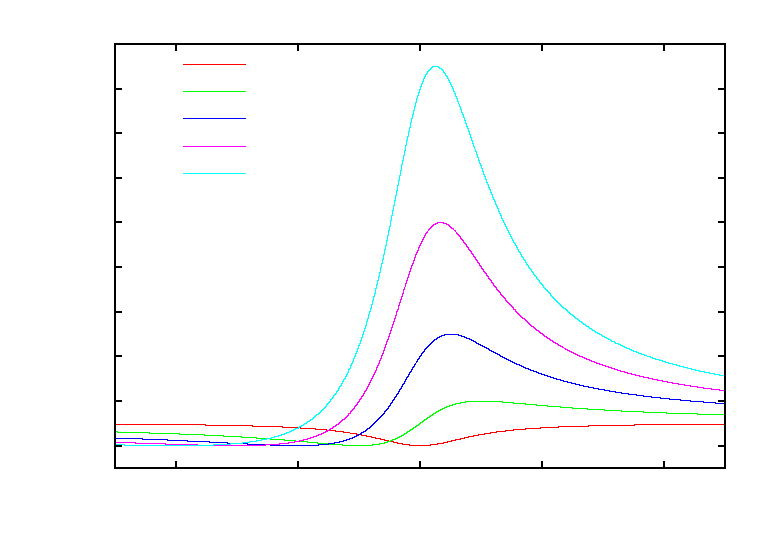
\includegraphics{fano}}%
    \gplfronttext
  \end{picture}%
\endgroup

	\caption[Fano-Profil]{Plot eines Fano-Profils gemäß Gl.
	\eqref{eq:fano-profil} mit $\Gamma=2$, $E_0=0$ und verschiedenen
	$q$.}
	\label{fig:fano}
\end{figure}
Man erkennt, dass es sowohl konstruktive (Maximum) als auch destruktive
(Minimum) Interferenzen zwischen den Übergängen in das Kontinuum und Übergänge
in einen diskreten Zustand gibt. Für den Fall $q=0$ findet man in Resonanz
bei $\epsilon=0$ ein Minimum, die sog. \textit{Window-Resonanz}. Für große $q$
ist dagegen die Überhöhung der Autoionisation gegenüber der nicht-resonanten
Photoionisation näherungsweise quadratisch in $q$ und $\sigma$ nähert sich einem Lorentzprofil.\par
Komplizierter wird die Beschreibung, wenn man mit einbezieht, dass verschiedene
Resonanzen und auch Kontinua miteinander interferieren. Dazu wird allgemein ein
Streuprozess betrachtet, bei dem das vor der Streuung gebundene Elektron am
Ion streut und für $t\to\infty$ sich ein freies Ion-Elektron-System ergibt. Dies
lässt sich gut mit der \textit{K-Matrix Theorie} beschreiben. Nach
\cite{connerade:1998:highly_excited_atoms} ergibt sich dann für den
Wirkungsquerschnitt
\begin{equation}\label{eq:k-matrix_wirkungsquerschnitt}
	\sigma\left(q_{1..n},\Gamma_{1..n},E_{1..n},E\right)=\abs{\tilde{D}}^2\frac{\left(1+\sum\limits_{k=1}^n{\frac{\nicefrac{\Gamma_k}{2}}{\left(E_k-E\right)}q_k}\right)^2}{1+\left(\sum\limits_{k=1}^n{\frac{\nicefrac{\Gamma_k}{2}}{\left(E_k-E\right)}}\right)^2}\,.
\end{equation}
Für zwei interferierende Resonanzen wurde der Wirkungsquerschnitt in Abb.
\ref{fig:k-matrix_wirkungsquerschnitt} aufgetragen.
\begin{figure}
	\centering
	\footnotesize
	% GNUPLOT: LaTeX picture with Postscript
\begingroup
  \makeatletter
  \providecommand\color[2][]{%
    \GenericError{(gnuplot) \space\space\space\@spaces}{%
      Package color not loaded in conjunction with
      terminal option `colourtext'%
    }{See the gnuplot documentation for explanation.%
    }{Either use 'blacktext' in gnuplot or load the package
      color.sty in LaTeX.}%
    \renewcommand\color[2][]{}%
  }%
  \providecommand\includegraphics[2][]{%
    \GenericError{(gnuplot) \space\space\space\@spaces}{%
      Package graphicx or graphics not loaded%
    }{See the gnuplot documentation for explanation.%
    }{The gnuplot epslatex terminal needs graphicx.sty or graphics.sty.}%
    \renewcommand\includegraphics[2][]{}%
  }%
  \providecommand\rotatebox[2]{#2}%
  \@ifundefined{ifGPcolor}{%
    \newif\ifGPcolor
    \GPcolortrue
  }{}%
  \@ifundefined{ifGPblacktext}{%
    \newif\ifGPblacktext
    \GPblacktexttrue
  }{}%
  % define a \g@addto@macro without @ in the name:
  \let\gplgaddtomacro\g@addto@macro
  % define empty templates for all commands taking text:
  \gdef\gplbacktext{}%
  \gdef\gplfronttext{}%
  \makeatother
  \ifGPblacktext
    % no textcolor at all
    \def\colorrgb#1{}%
    \def\colorgray#1{}%
  \else
    % gray or color?
    \ifGPcolor
      \def\colorrgb#1{\color[rgb]{#1}}%
      \def\colorgray#1{\color[gray]{#1}}%
      \expandafter\def\csname LTw\endcsname{\color{white}}%
      \expandafter\def\csname LTb\endcsname{\color{black}}%
      \expandafter\def\csname LTa\endcsname{\color{black}}%
      \expandafter\def\csname LT0\endcsname{\color[rgb]{1,0,0}}%
      \expandafter\def\csname LT1\endcsname{\color[rgb]{0,1,0}}%
      \expandafter\def\csname LT2\endcsname{\color[rgb]{0,0,1}}%
      \expandafter\def\csname LT3\endcsname{\color[rgb]{1,0,1}}%
      \expandafter\def\csname LT4\endcsname{\color[rgb]{0,1,1}}%
      \expandafter\def\csname LT5\endcsname{\color[rgb]{1,1,0}}%
      \expandafter\def\csname LT6\endcsname{\color[rgb]{0,0,0}}%
      \expandafter\def\csname LT7\endcsname{\color[rgb]{1,0.3,0}}%
      \expandafter\def\csname LT8\endcsname{\color[rgb]{0.5,0.5,0.5}}%
    \else
      % gray
      \def\colorrgb#1{\color{black}}%
      \def\colorgray#1{\color[gray]{#1}}%
      \expandafter\def\csname LTw\endcsname{\color{white}}%
      \expandafter\def\csname LTb\endcsname{\color{black}}%
      \expandafter\def\csname LTa\endcsname{\color{black}}%
      \expandafter\def\csname LT0\endcsname{\color{black}}%
      \expandafter\def\csname LT1\endcsname{\color{black}}%
      \expandafter\def\csname LT2\endcsname{\color{black}}%
      \expandafter\def\csname LT3\endcsname{\color{black}}%
      \expandafter\def\csname LT4\endcsname{\color{black}}%
      \expandafter\def\csname LT5\endcsname{\color{black}}%
      \expandafter\def\csname LT6\endcsname{\color{black}}%
      \expandafter\def\csname LT7\endcsname{\color{black}}%
      \expandafter\def\csname LT8\endcsname{\color{black}}%
    \fi
  \fi
  \setlength{\unitlength}{0.0500bp}%
  \begin{picture}(7200.00,5040.00)%
    \gplgaddtomacro\gplbacktext{%
      \csname LTb\endcsname%
      \put(1342,704){\makebox(0,0)[r]{\strut{} 1000}}%
      \put(1342,1937){\makebox(0,0)[r]{\strut{} 10000}}%
      \put(1342,3171){\makebox(0,0)[r]{\strut{} 100000}}%
      \put(1342,4404){\makebox(0,0)[r]{\strut{} 1e+006}}%
      \put(1474,484){\makebox(0,0){\strut{}-100}}%
      \put(2235,484){\makebox(0,0){\strut{} 0}}%
      \put(2997,484){\makebox(0,0){\strut{} 100}}%
      \put(3758,484){\makebox(0,0){\strut{} 200}}%
      \put(4519,484){\makebox(0,0){\strut{} 300}}%
      \put(5280,484){\makebox(0,0){\strut{} 400}}%
      \put(6042,484){\makebox(0,0){\strut{} 500}}%
      \put(6803,484){\makebox(0,0){\strut{} 600}}%
      \put(176,2739){\rotatebox{-270}{\makebox(0,0){\strut{}$\sigma$}}}%
      \put(4138,154){\makebox(0,0){\strut{}E}}%
    }%
    \gplgaddtomacro\gplfronttext{%
      \csname LTb\endcsname%
      \put(2794,4581){\makebox(0,0)[r]{\strut{}$q_1=50$}}%
      \csname LTb\endcsname%
      \put(2794,4318){\makebox(0,0)[r]{\strut{}$q_1=100$}}%
      \csname LTb\endcsname%
      \put(2794,4055){\makebox(0,0)[r]{\strut{}$q_1=200$}}%
      \csname LTb\endcsname%
      \put(2794,3792){\makebox(0,0)[r]{\strut{}$q_1=300$}}%
      \csname LTb\endcsname%
      \put(2794,3529){\makebox(0,0)[r]{\strut{}$q_1=400$}}%
    }%
    \gplbacktext
    \put(0,0){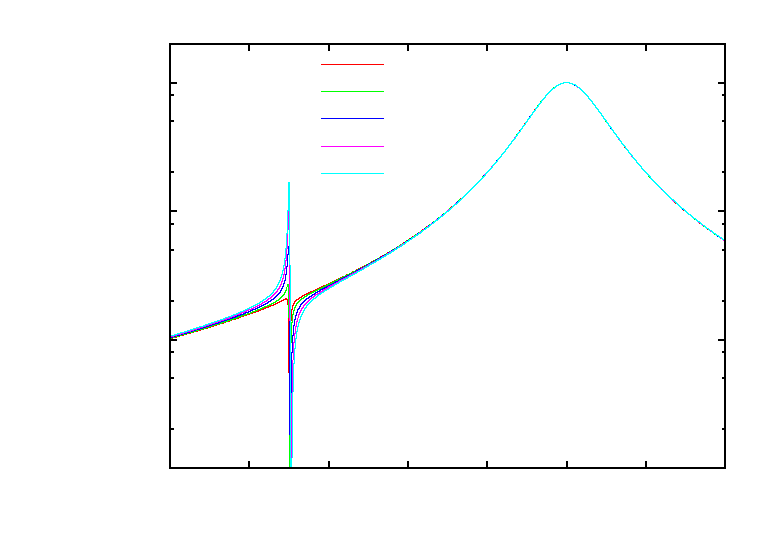
\includegraphics{k-matrix_wirkungsquerschnitt}}%
    \gplfronttext
  \end{picture}%
\endgroup

	\caption[Wirkungsquerschnitt - K-Matrix Theorie]{Plot des Wirkungsquerschnitts
	gemäß Gl. \eqref{eq:k-matrix_wirkungsquerschnitt} mit $q_2=1000$, $E1=50$,
	$E2=400$, $\Gamma_1=2$, $\Gamma_2=2$ und verschiedenen $q_1$.}
	\label{fig:k-matrix_wirkungsquerschnitt}
\end{figure}
Danach haben schmale Resonanzen ein asymmetrisches Fano-Profil, wenn sie durch
eine benachbarte breite Resonanz gestört werden. Auch zu erkennen ist, dass
Resonanzen mit relativ zu anderen Resonanzen kleinem $q$ wie Window-Resonanzen
erscheinen.

\subsection{Isotopieverschiebung}\label{subsec:isotopieverschiebung}
Aufgrund der verschiedenen Kerneigenschaften der Isotope eines Elements kommt es
zu Energieniveauverschiebungen:
\begin{equation}\label{eq:isotopieshift}
	\delta\nu_{IV}=\delta\nu_{ME}+\delta\nu_{FE}\,.
\end{equation}
Diese Verschiebungen liegen zwischen einigen $100\,$MHz und einigen GHz. In
Relation zur Gesamtenergie eines Niveaus, welches bei einigen $100\,$THz liegt,
sind diese Verschiebungen zwar klein, aber mit schmalbandigen Lasern gut
auflösbar. Dadurch können Isotope selektiv angeregt werden.
Die Verschiebung ist zum einen durch die Massenänderung und zum anderen durch die veränderte Ladungsverteilung des Kerns zu begründen (Masseneffekt $\delta\nu_{ME}$ und Feldeffekt $\delta\nu_{FE}$ in \eqref{eq:isotopieshift}). Der Masseneffekt
\begin{equation}\label{eq:masseneffekt}
	\delta\nu_{ME}=K_{ME}\frac{m_{A'}-m_A}{m_{A'}m_A}
\end{equation}
ist von den beiden Massen $m_{A'}$ und $m_A$ der Isotope und von der
Masseneffektkonstante $K_{ME}=K_{NME}+K_{SME}$ abhängig. Die
Masseneffektkonstante wiederum besteht aus dem normalen Masseneffekt
\begin{equation}\label{eq:normaler_masseneffekt}
	\delta\nu_{NME}=m_e\nu_A\frac{m_A}{m_A+m_e}\,,
\end{equation}
der aus der veränderten reduzierten Masse, die sich in einem
Ein-Elektronen-System ergeben würde, resultiert und dem spezifischen
Masseneffekt $K_{SME}$, der aus der Änderung der Korrelation aller
Elektronenimpulse folgt und bestenfalls nur numerisch abgeschätzt werden
kann. \par
Da die Ortsanteile der Wellenfunktionen der Elektronen mit Bahndrehimpuls
$l=0$ mit dem Ort des Kerns überlappen, kommt es bei Veränderung der
Kernladungsdichteverteilung auch zu einer Energieniveauverschiebung:
\begin{equation}\label{eq:feldeffekt}
	\delta\nu_{FE}=K_{FE}\delta\mean{r^2}\,.
\end{equation}
Mit der Annahme, dass die Wellenfunktionen der Elektronen am Ort des Kerns
nicht stark variieren und in jedem Isotop die gleiche sphärische Symmetrie
vorliegt, kann die Änderung der Kernladungsdichteverteilung nach geraden
Potenzen entwickelt werden. In Gl. \eqref{eq:feldeffekt} wurde
die quadratische (niedrigste) Ordnung dieser Entwicklung eingesetzt.\par
Generell unterscheidet man zwischen der \textit{level-isotope-shift}
(LIS) und der \textit{transition-isotope-shift} (TIS). Bei ersterer betrachtet
man die Energieverschiebung eines Zustands zwischen den Isotopen in Relation zum
jeweiligen Grundzustandsniveau:
\begin{equation}\label{eq:LIS}
	\delta\nu_{IV}^{LIS}(E)=\nu_{A_1}^{GZ_1\leftrightarrow
	E}-\nu_{A_2}^{GZ_2\leftrightarrow E}\,.
\end{equation}
Der TIS ist durch die Verschiebung des Abstands zweier Energieniveaus definiert:
\begin{equation}\label{eq:TIS}
	\delta\nu_{IV}^{TIS}(E',E)=\nu_{A_1}^{E'\leftrightarrow
	E}-\nu_{A_2}^{E'\leftrightarrow E}\,.
\end{equation}
Dies ist die in der Praxis nützlichere Definition, da sie die Verschiebung
angibt, die das Laserlicht verstimmt werden muss, um
den gleichen Übergang zum Anregen verschiedener Isotope zu verwenden. LIS und
TIS sind über
\begin{equation}\label{eq:TIS_LIS_verknuepfung}
	\delta\nu_{IV}^{TIS}(E',E)=\delta\nu_{IV}^{LIS}(E)-\delta\nu_{IV}^{LIS}(E')
\end{equation}
miteinander verknüpft.

\section{Diodenlaser in der RIS}\label{sec:diodenlaser}
Um hochaufgelöste Spektroskopie oder hochselektive Isotopentrennung
durchzuführen, sind schmalbandige Laser nötig. Die ebenfalls in der AG Larissa
verwendeten gepulst betriebenen Ti:Sa-Laser (Festkörperlaser) haben neben dem
Vorteil hoher Leistung und großen Durchstimmbereichs von bis zu $300\,$nm den
Nachteil großer Linienbreite von $3$-$5\,$GHz.\par
Als schmalbandige Laser kommen Diodenlaser zum Einsatz, deren typische
Linienbreiten bei wenigen MHz liegen. Ihre spektralen Betriebsbereiche sind
wenige nm im blauen und bis zu $50\,$nm im roten Spektralbereich. Mithilfe eines externen Resonators können Diodenlaser bis zu $30\,$GHz kontinuierlich
verstimmt werden, was zur Abdeckung der Isotopieverschiebungen und für
hochauflösenden Spektroskopie ausreichend ist.\par
Im Folgenden soll die Funktionsweise der hier verwendeten Diodenlaser erklärt
werden. Die dabei verwendete Literatur besteht weitestgehend aus den Lehrbüchern
\cite{demtroeder:ex3}, \cite{chow:semiconductor-laser} und der Arbeit
\cite{schumann:2001:diplomarbeit}.

\subsection{Prinzip des Halbleiterlasers}\label{subsec:prinzip_halbleiterlaser}
Wie in Abschn. \ref{sec:licht-atom-wechselwirkung} bereits ausführlich erklärt
wurde, treten bei der Licht-Atom-Wechselwirkung die drei Prozesse
\textit{Absorption}, \textit{stimulierte Emission} und \textit{spontane Emission} auf. Auch wurde
gezeigt, dass in einem rein optisch betriebenen Zwei-Niveau-System keine
Besetzungsinversion möglich ist.
Möchte man allerdings in dem sog. \textit{aktiven Medium} eines Lasers eine Lichtverstärkung
hervorrufen, muss die Emissionsrate die Absorptionsrate überwiegen. Das aktive Medium ist der von einem Resonator
umgebene Bereich eines Lasers, in dem durch stimulierte Emission eine
Verstärkung des Lichtfelds hervorgerufen wird. Dabei stammt das stimulierende
Lichtfeld vom getriebenen Übergang des selben aktiven Mediums und bildet eine
stehende bzw. fortlaufende Welle in einem Fabry-Perot- bzw. Ring-Resonator aus.
Ein Teil des Lichts im Resonator wird als Nutzlicht ausgekoppelt. Der andere Teil wird zur Verstärkung verwendet. Eine
Besetzungsinversion liegt dann vor, wenn die Besetzungswahrscheinlichkeit des
angeregten Zustands größer als $50\%$ ist.
Da durch rein optisches Pumpen in einem
2-Niveau-System keine Besetzungsinversion möglich ist, kann beispielsweise
elektrisch gepumpt werden, was mit Halbleitern möglich ist und in Abschn.
\ref{subsec:halbleiterlaser} näher beschrieben wird. Alternativ kann in
Lasermedien auch mit Blitzlichtlampen gepumpt werden. In rein optisch gepumpten
Lasern werden zur Besetzungsinversion eines Übergangs mehrere Niveaus benötigt,
worauf an dieser Stelle allerdings nicht weiter eingegangen werden soll. In Abb.
\ref{fig:halbleiterlaser-prinzip} ist noch einmal schematisch das Prinzip eines
Halbleiterlasers/Diodenlasers dargestellt.
\begin{figure}[h]
	\centering
	\fbox{
		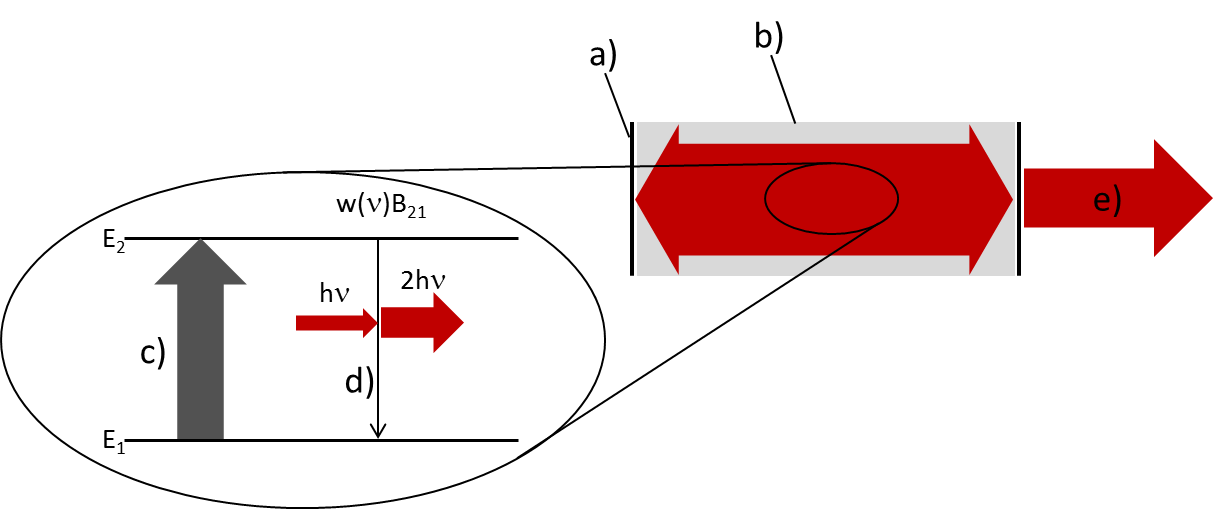
\includegraphics[width=\textwidth-1cm]{gfx/halbleiterlaser-prinzip}
	}
	\caption[Halbleiterlaser Prinzip]{Halbleiterlaser-Prinzip: a) Resonatorwände
	rechts und links (Spiegel); b) aktives Medium; c) elektrisches Pumpen; d)
	stimulierte Emission; e) Nutzlicht.
	Erklärungen im Text.}
	\label{fig:halbleiterlaser-prinzip}
\end{figure}

\subsection{Halbleiterlaser: Bauarten und
Funktion}\label{subsec:halbleiterlaser}
In diesem Kapitel wird das Verständnis des \textit{Bändermodells} vorausgesetzt.
Dabei sei auf das Lehrbuch \cite{demtroeder:ex3} verwiesen.\par
Als Übergang in
einem Halbleiterlaser bedient man sich zweier benachbarter Energiebänder, die
als Vier-Niveau-System angesehen werden
können und deren Bandlücke der Energie des emittierten Lichts entspricht.
Das energetisch höher liegende Band wird \textit{Leitungsband}, das untere
\textit{Valenzband} genannt, wobei die Bänder so gewählt sind, dass das
Ferminiveau dazwischen liegt. Dies bedeutet, dass das Valenzband im Grundzustand
bei $T=0$ noch mit Ladungsträgern besetzt ist, das
Leitungsband jedoch nicht. Für $T>0$ verschmiert diese diskrete
Energiegrenze. Ein typisches Halbleiterelement ist Silicium, welches vier
Valenzelektronen besitzt. Durch Einbringen von Donatoren bzw.
Akzeptoren, Elementen mit einem Valenzelektron mehr bzw. weniger, kann man
Halbleiter negativ bzw. positiv dotieren. Die Grundzustände der Donatoren bzw. Akzeptoren liegen unterhalb des
Leitungs- bzw. oberhalb des Valenzbandes (siehe
\ref{fig:pn-halbleiter}\subref{subfig:pn-halbleiter_a}).
\begin{figure}[h]
 	\centering
 	\fbox{\parbox{\dimexpr \linewidth - 2\fboxrule - 2\fboxsep}{
		\subfloat[]{
			\label{subfig:pn-halbleiter_a}
	    	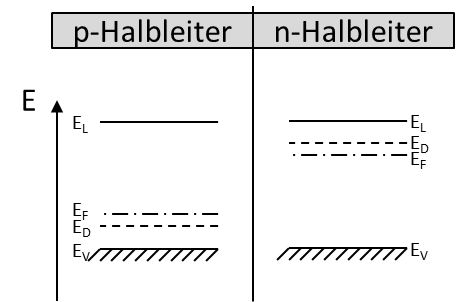
\includegraphics[width=(\textwidth-1cm)/2]{gfx/pn-halbleiter_a}
	  	}
		\subfloat[]{
			\label{subfig:pn-halbleiter_b}
	    	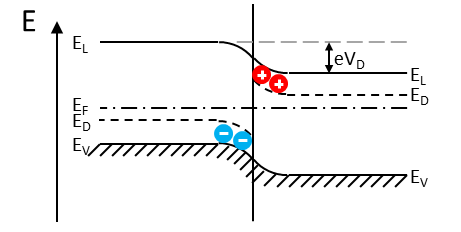
\includegraphics[width=(\textwidth-1cm)/2]{gfx/pn-halbleiter_b}
	  	}\\
	  	\subfloat[]{
			\label{subfig:pn-halbleiter_c}
	    	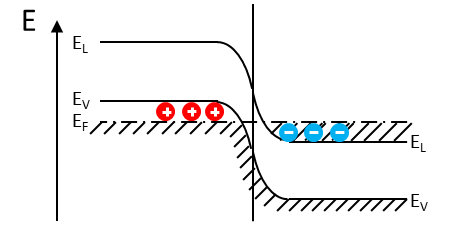
\includegraphics[width=(\textwidth-1cm)/2]{gfx/pn-halbleiter_c}
	  	}
		\subfloat[]{
			\label{subfig:pn-halbleiter_d}
	    	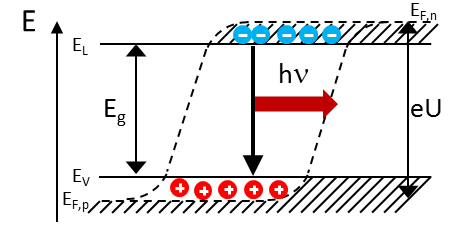
\includegraphics[width=(\textwidth-1cm)/2]{gfx/pn-halbleiter_d}
	  	}
	}}
	\caption[Bandstruktur Halbleiterlaser]{Bandstruktur eines
	p-n-Halbleiters mit der Fermienergie $E_F$, der Ober- bzw. Untergrenze des Valenz- bzw.
	Leitungsbandniveau $E_V$ bzw. $E_L$ und dem Akzeptor- bzw. Donatorniveau $E_A$
	und $E_D$:
	(a) Energieniveaus mit Dotierung; (b) Energieniveaus nach
	Zusammenführen der p- und n-Schicht; (c) starke
	Dotierung; (d) mit angelegter Mindestspannung $U$
	(Laserbetrieb). Erklärungen im
	Text.}
	\label{fig:pn-halbleiter}
\end{figure}
Somit stellt
man im n-dotierten Halbleiter frei bewegliche Elektronen und im p-dotierten Halbleiter frei bewegliche positive
Ladungsträger, auch \textit{Löcher} genannt, zur Verfügung
(\textit{Majoritätsladungsträger}). Beim Zusammenbringen von n- und p-dotierten
Halbleitern entsteht ein Konzentrationsgradient der
Ladungsträger. Durch die Diffusionskraft diffundieren die
Majoritätsladungsträger in den jeweils andere Halbleiter, wo sie dann
\textit{Minoritätsladungsträger} genannt werden. Somit entsteht in der
Grenzregion im Gleichgewicht ein sog. \textit{Makropotential} mit der \textit{Diffusionsspannung} $V_D$. Da
das Ferminiveau als chemisches Potential in beiden Teilen des Halbleiters gleich
sein muss, verschieben sich die Bänder um $eV_D$ (siehe
\ref{fig:pn-halbleiter}\subref{subfig:pn-halbleiter_b}). Bei starker Dotierung
liegt das Ferminiveau unter dem Valenzband des p-dotierten Bereichs und über dem Leitungsbandes des
n-dotierten Bereichs, was bedeutet, dass das Valenzband des p-dotierten Bereichs
stark mit Löchern und das Leitungsband des n-dotierten Bereichs stark mit
Elektronen besetzt ist (siehe
\ref{fig:pn-halbleiter}\subref{subfig:pn-halbleiter_c}). Legt man nun eine Spannung $U$ an, die die Niveauverschiebung der beiden Halbleiterteile
kompensiert, können die Elektronen im Leitungsband des n-dotierten Bereichs mit
den Löchern im Valenzband des p-dotierten Bereichs rekombinieren, was mit der
Emission von Photonen verbunden sein kann (siehe
\ref{fig:pn-halbleiter}\subref{subfig:pn-halbleiter_d}).
Beim Anlegen der Spannung entstehen \textit{Quasi-Ferminiveaus} $E_F^n$ und $E_F^p$ der beiden Dotierungen mit
\begin{equation}\label{eq:quasi-ferminiveaus}
	U=\frac{\left(E_F^n-E_F^p\right)}{e}\,.
\end{equation}
Die Endspiegel des Resonators werden durch die Abschlussflächen des
Halbleiterkristalls mit einer Reflektivität von ca. $30\,\%$ realisiert, wobei der Resonator
zwischen den n- und p-Schichten typischerweise etwa $1\,$µm dick, $10\,$µm breit
und $250\,$µm lang ist. Um die durch Rekombination verarmenden Niveaus wieder aufzufüllen,
muss ein konstanter Strom fließen.

\subsubsection{Heteostrukturen}\label{heterostrukturen}
Die ersten Halbleiterlaser bestanden nur aus einer n- und einer
p-Schicht. Die Laser mussten weit unter Raumtemperatur mit einer hohen
\textit{Schwellenstromdichte} gepulst betrieben werden. Ihre Lebensdauer betrug
nur wenige Minuten. Um zu verstehen, wie die Schwellenstromdichte mit den
Laserparametern verknüpft ist, betrachtet man die Bedingung
\begin{equation}\label{eq:schwellenbedingung}
	R_1R_2\mathrm{e}^{2\left(\Gamma G_{th}-\alpha_{abs}\right)L}=1\,,
\end{equation}
für die Schwellenverstärkung $G_{th}$, bei der die optischen Verluste bei einem
Umlauf im Resonator gerade durch die Verstärkung ausgeglichen werden.
Dabei sind $R_1$ und $R_2$ die Reflektivitäten der Endspiegel, $\Gamma$ der
Confinement-Faktor, der die Güte des Überlapps von aktivem Medium und
Stehwelle charakterisiert, $\alpha_{abs}$ der Absorptionskoeffizient im
Medium und $L$ die Länge des aktiven Mediums. Aus dieser Bedingung folgt die
Schwellenverstärkung
\begin{equation}\label{eq:schwellenverstärkung}
	G_{th}=\frac{1}{\Gamma}\left(\alpha_{abs}-\frac{\mathrm{ln}{(R_1R_2)}}{2L}\right)\,.
\end{equation}
Die Verstärkung
\begin{equation}\label{eq:laser-verstärkung}
	G=A_g\left(N-N_g\right)
\end{equation}
ergibt sich in guter Näherung aus dem Verstärkungskoeffizienten $A_g$ und der
Schwellenladungsträgerdichte $N_g$, die beide von Materialeigenschaften abhängig
sind. Die Ladungsträgerdichte
\begin{equation}\label{eq:ladungstraegerdichte}
	N=\frac{J\eta}{e\gamma_{nr}d}
\end{equation}
erhält man aus der Elementarladung $e$, der Rekombinationsrate $\gamma_{nr}$,
der Dicke des aktiven Mediums $d$, der Quanteneffizienz der Inversion $\eta$ und der
Stromdichte $J$. Insgesamt findet man dann für die Schwellenstromdichte
\begin{equation}\label{eq:schwellenstromdichte}
	J_{th}=\frac{e\gamma_{nr}d}{\eta}\left[N_g+\frac{\alpha_{abs}-\nicefrac{\mathrm{ln}{\left(R_1R_2\right)}}{2L}}{A_g\Gamma}\right]\,.
\end{equation}
Hieraus ist ersichtlich, dass durch Verkleinerung der aktiven Schicht die
Schwellenstromdichte verringert werden kann. Zum einen können die
Brechungsindizes räumlich so verändert werden, dass sie durch Totalreflexion die
aktive Schicht weiter einengen (\textit{optical confinement}). Zum anderen ist
es möglich, durch bestimmte Strukturen der Bandenergien einen engeren Einschluss
der Ladungsträger zu erreichen (\textit{electrical confinement}). In sog.
\textit{Heterostrukturen} werden diese beiden Effekte ausgenutzt, in dem man
mehrere Schichten von dotierten Halbleitern kombiniert. Dabei ist darauf zu
achten, dass sich die verschiedenen Kristalle in der Struktur ähneln, damit
möglichst keine Störstellen entstehen. In Abb. \ref{fig:heterostrukturen} sind
einige Heterostrukturen sowie die zugehörigen Bandlücke und Brechungsindizes
dargestellt. Durch die Einengung der aktiven Schicht konzentriert sich auch
entsprechend die Ausstrahlung $M$, wie Abb. \ref{fig:heterostrukturen} zeigt.
Laserdioden mit der zunächst einmal eindimensionalen Einengung senkrecht zu den Schichten nennt man \textit{kantenemittierende} Laserdioden.
\begin{figure}[h]
	\centering
	\fbox{
		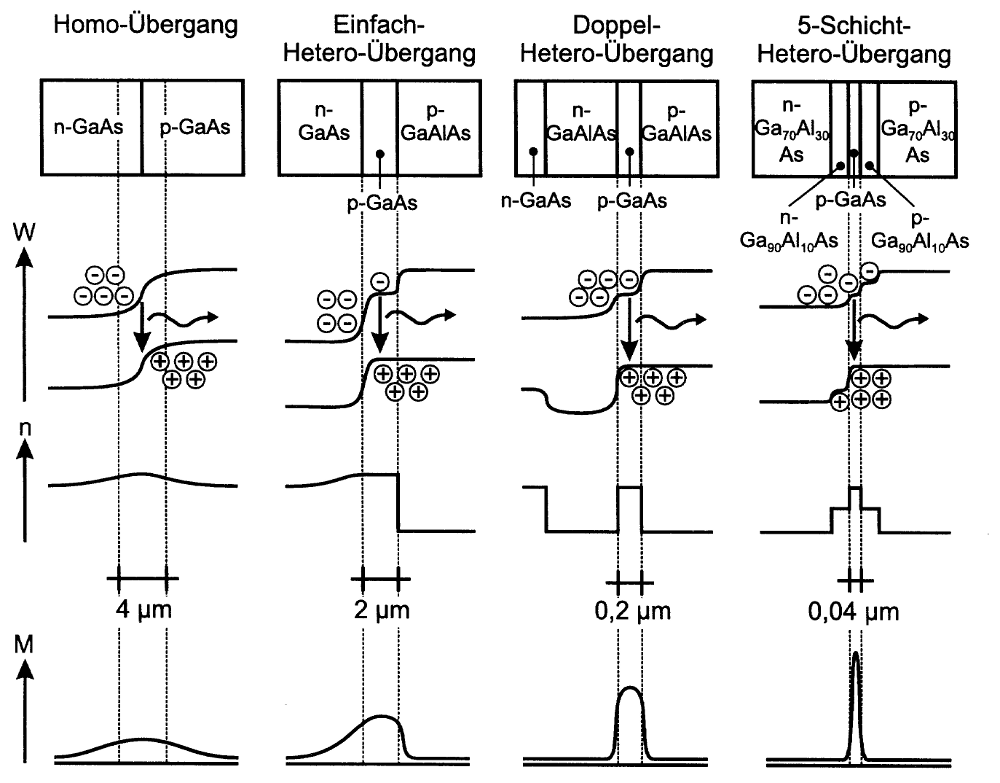
\includegraphics[width=\textwidth-1cm]{gfx/heterostrukturen}
	}
	\caption[Heterostrukturen]{Verschiedene Heterostrukturen von
	Halbleiterlasern. Dargestellt sind Schichtaufbau,
	Bandstruktur $W$, Verlauf des Brechungsindex $n$ 
	und spezifische Ausstrahlung $M$. (aus
	\cite{schumann:2001:diplomarbeit})}
	\label{fig:heterostrukturen}
\end{figure}

\subsubsection{Lasermoden}\label{subsubsec:lasermoden}
Wie schon erwähnt, kann der Resonator des Lasers durch Totalreflexion an den
Schichtgrenzen realisiert werden. Dabei ist der Resonator allerdings nur in
einer Dimension begrenzt. Eine Möglichkeit für die transversale Eingrenzung in
der Schichtenebene ist eine lokal begrenzte Stromzuführung, auch \textit{gain
guided laser} bzw. \textit{gewinngeführter Laser} genannt. Alternativ ist es
möglich, transversal verschieden dotierte Schichten einzubringen, wodurch, wie
bei der lateralen Einengung unterschiedliche Brechungsindizes Totalreflexion
bewirken (\textit{index guided laser} bzw. \textit{indexgeführter Laser}). Beide
Varianten sind in Abb. \ref{fig:transversale_eingrenzung_diodenlaser}
dargestellt.
\begin{figure}[h]
 	\centering
 	\fbox{\parbox{\dimexpr \linewidth - 2\fboxrule - 2\fboxsep}{
		\subfloat[]{
			\label{subfig:transversale_eingrenzung_diodenlaser_a}
	    	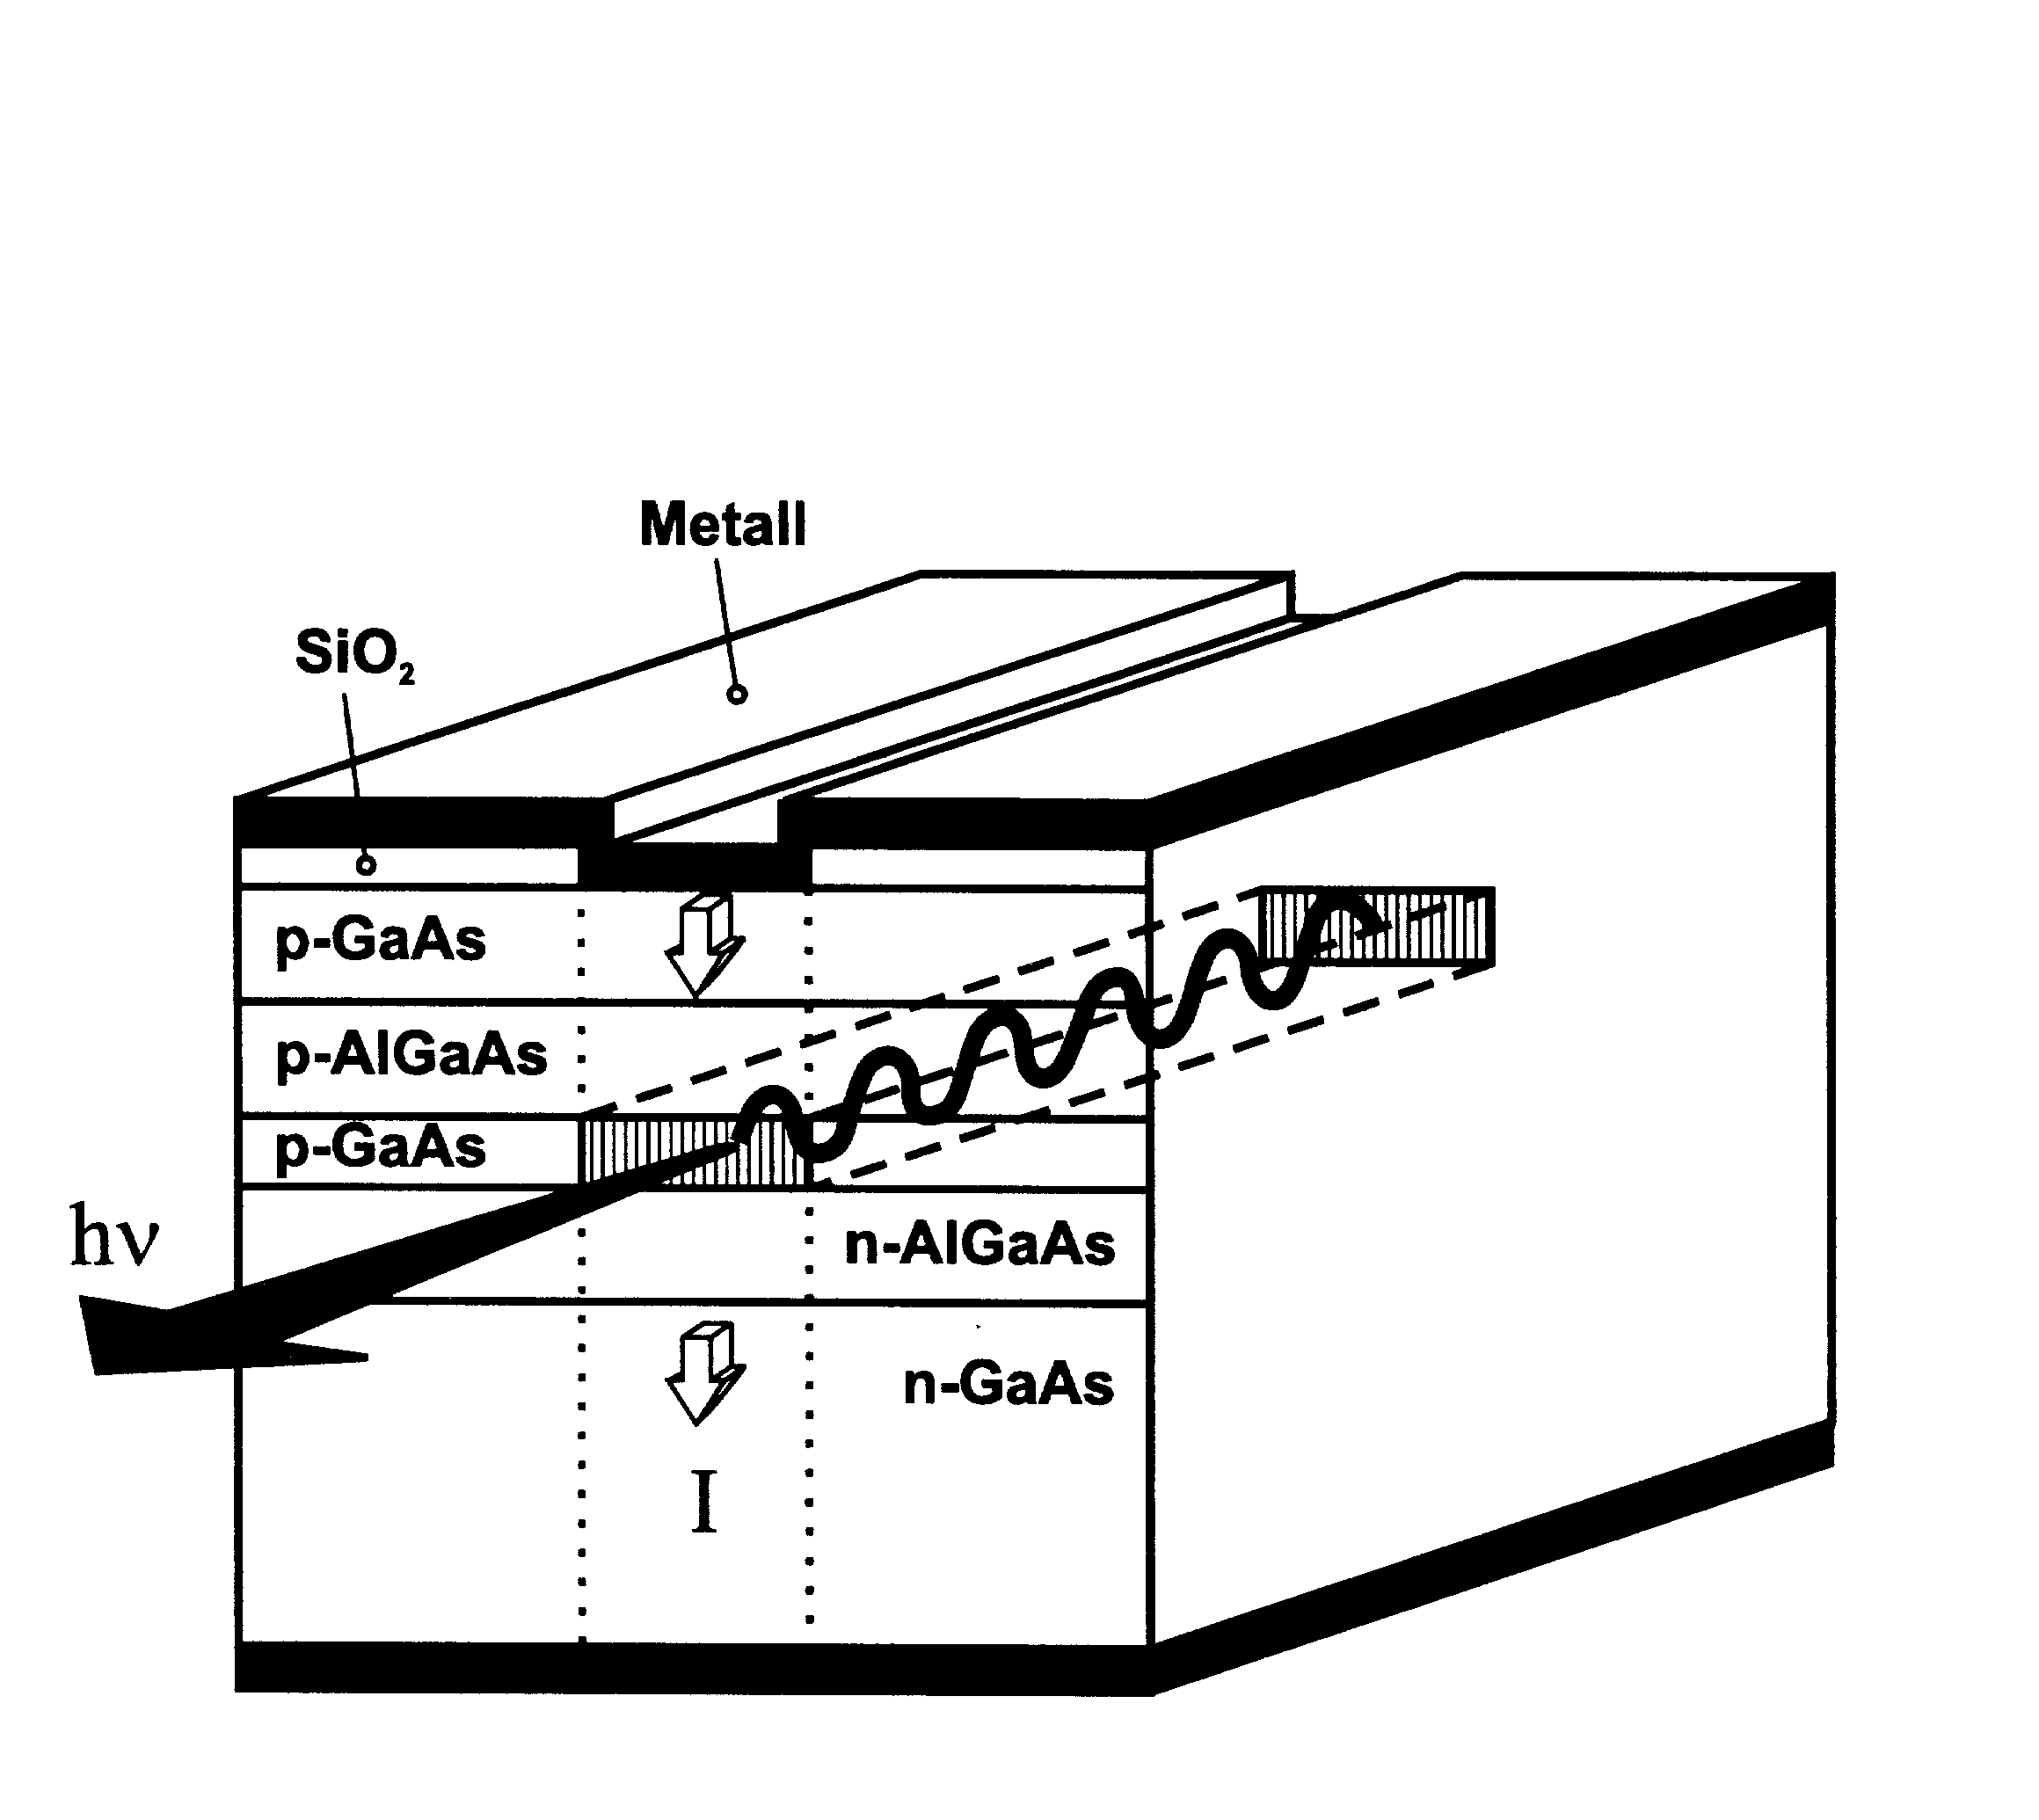
\includegraphics[width=(\textwidth-1cm)/2]{gfx/transversale_eingrenzung_diodenlaser_a}
	    	}
		\subfloat[]{
			\label{subfig:transversale_eingrenzung_diodenlaser_b}
	    	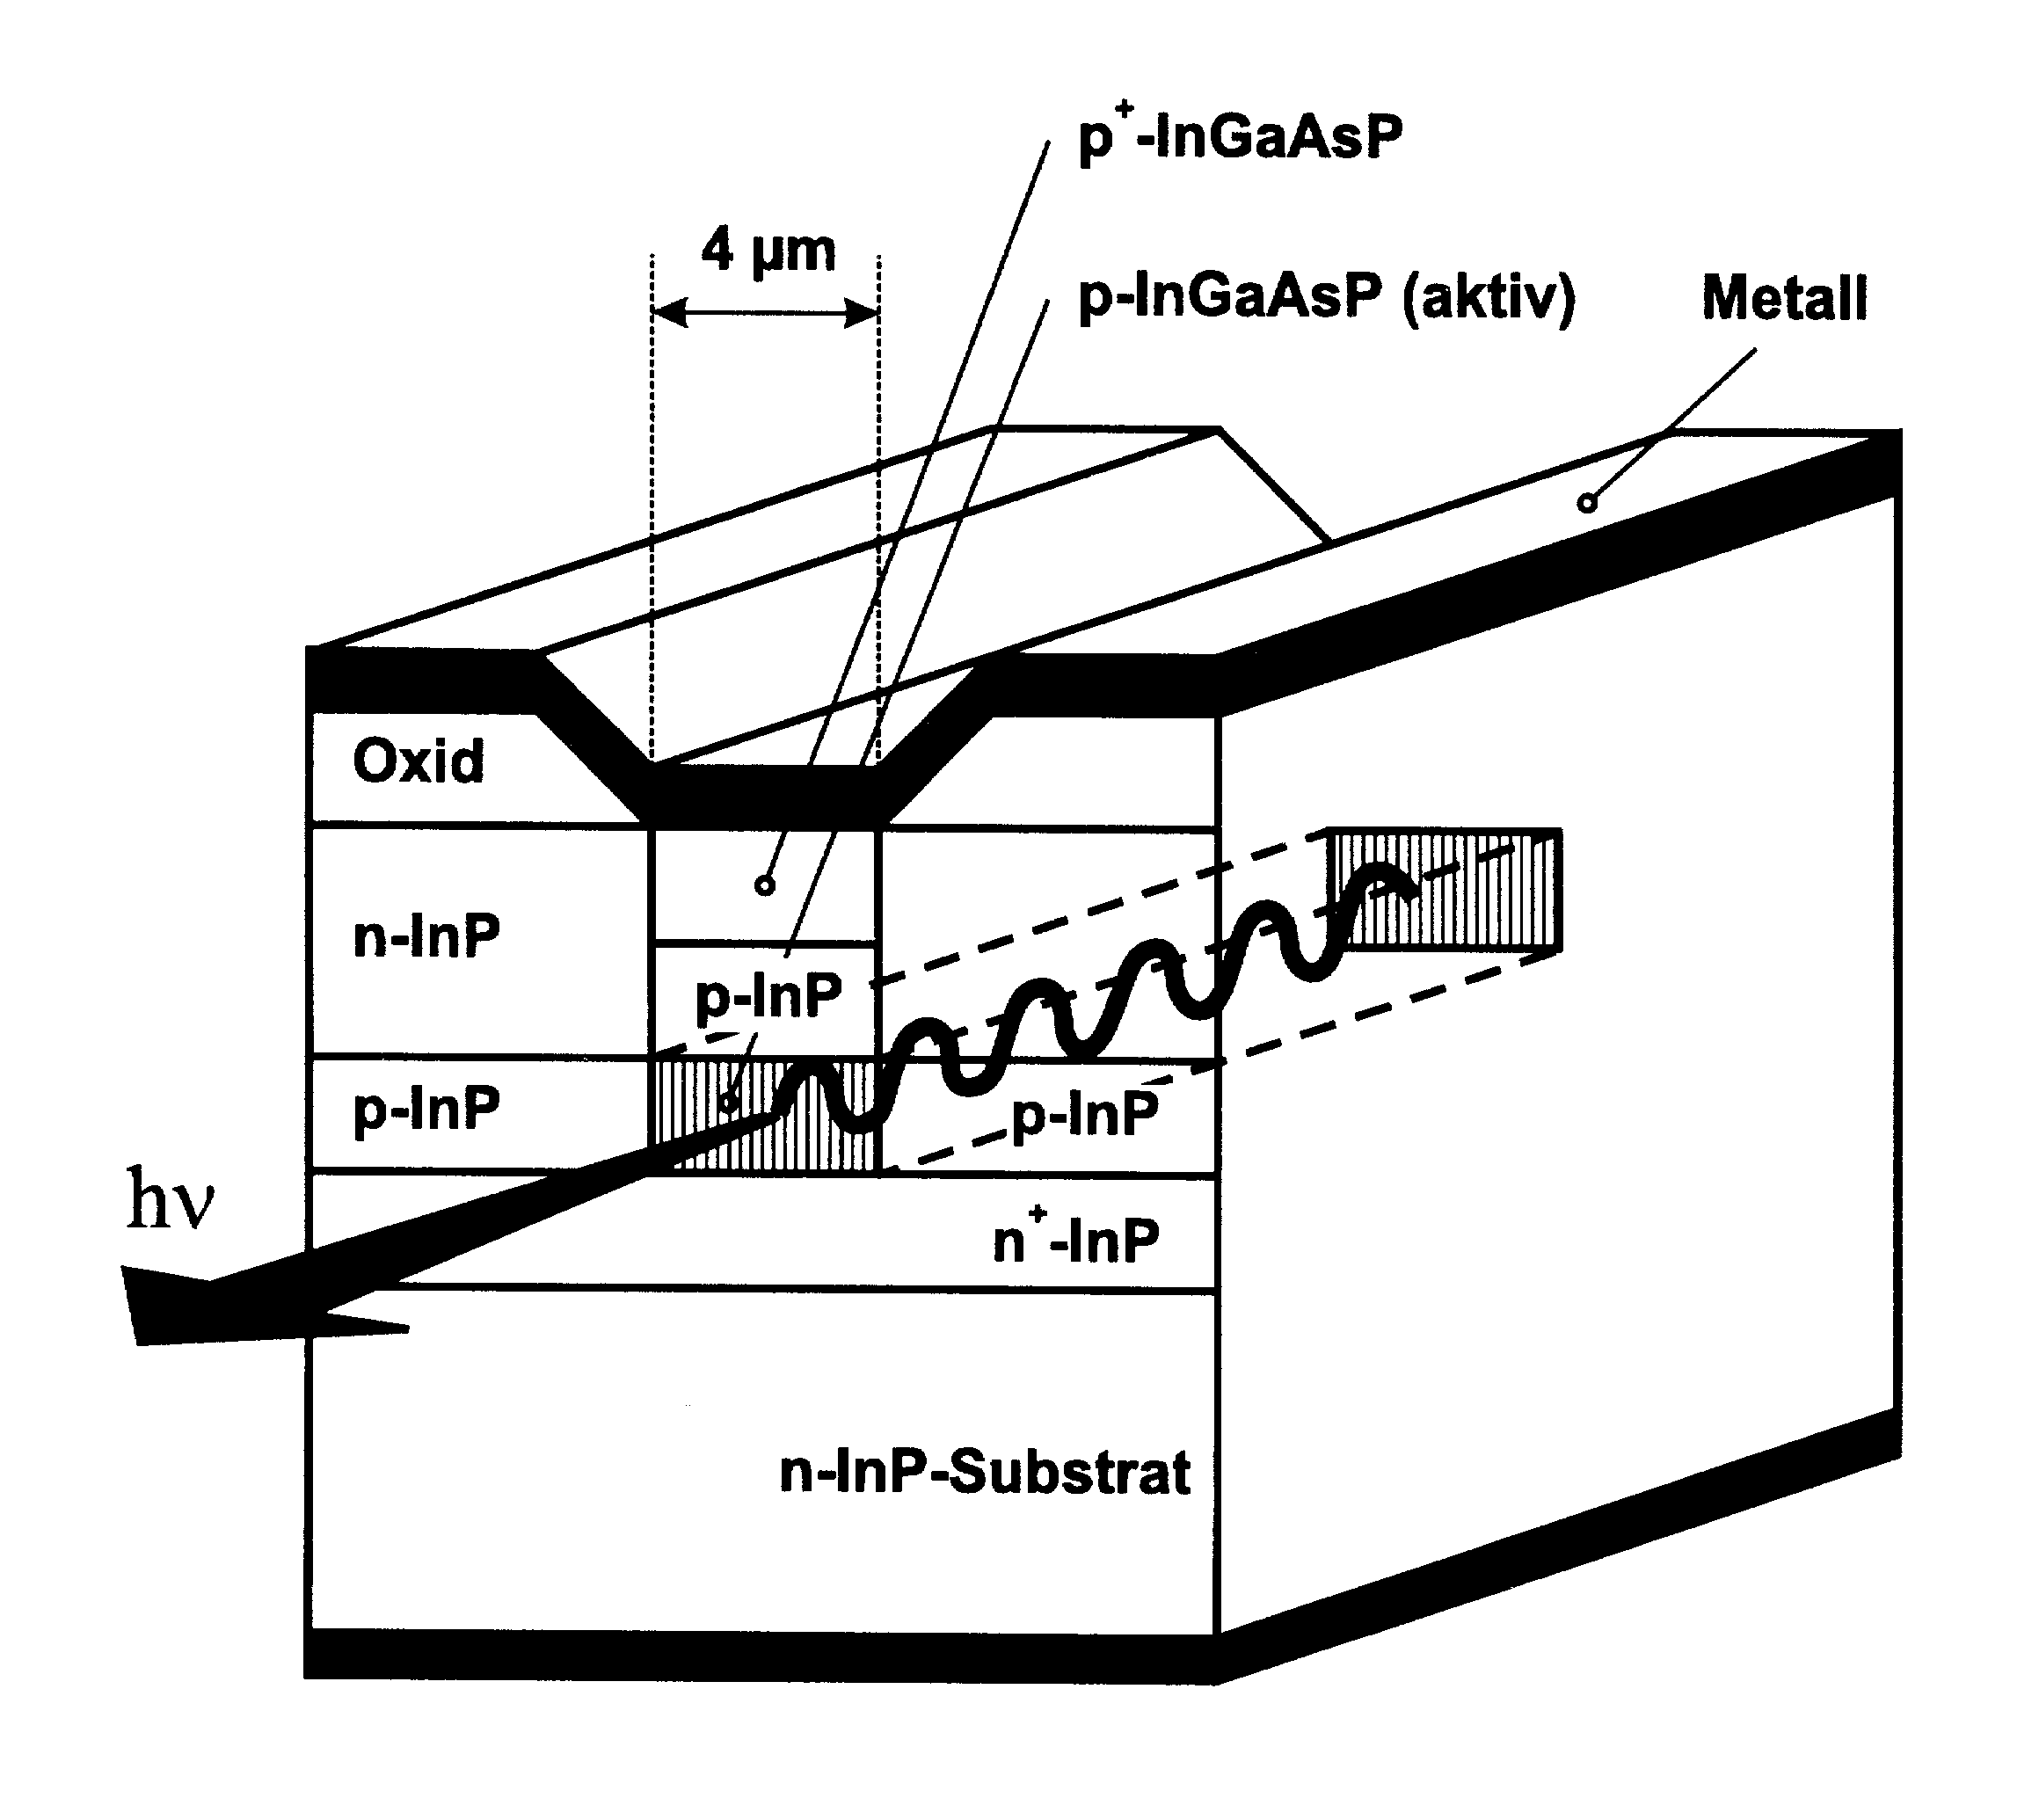
\includegraphics[width=(\textwidth-1cm)/2]{gfx/transversale_eingrenzung_diodenlaser_b}
	    	}
  	}}
	\caption[Gewinn- und indexgeführte Laserdiode]{Aufbauten
	einer gewinngeführten (a) und indexgeführten (b), kantenemittierenden
	Laserdiode. Der aktive Bereich ist der schraffierte Bereich.
	(aus \cite{schumann:2001:diplomarbeit})}
	\label{fig:transversale_eingrenzung_diodenlaser}
\end{figure}
In einem solchen offenen Resonator bilden sich sog.
\textit{transversal-elektromagnetische Moden}, kurz TEM$_{mn,q}$, aus, wobei $m$
und $n$ die zur Resonatorachse senkrechten Ordnungen und $q$ die longitudinale
Ordnung indizieren. Die Ordnung ist durch die Anzahl der ausgebildeten
Stehwellenknoten in der jeweiligen Raumrichtung definiert. In
Abb. \ref{fig:TEM-moden} ist die Amplitude der fundamentalen Mode, der erste und
der zweite Harmonische einer Raumrichtung dargestellt.
\begin{figure}[h]
	\centering
	\footnotesize
	% GNUPLOT: LaTeX picture with Postscript
\begingroup
  \makeatletter
  \providecommand\color[2][]{%
    \GenericError{(gnuplot) \space\space\space\@spaces}{%
      Package color not loaded in conjunction with
      terminal option `colourtext'%
    }{See the gnuplot documentation for explanation.%
    }{Either use 'blacktext' in gnuplot or load the package
      color.sty in LaTeX.}%
    \renewcommand\color[2][]{}%
  }%
  \providecommand\includegraphics[2][]{%
    \GenericError{(gnuplot) \space\space\space\@spaces}{%
      Package graphicx or graphics not loaded%
    }{See the gnuplot documentation for explanation.%
    }{The gnuplot epslatex terminal needs graphicx.sty or graphics.sty.}%
    \renewcommand\includegraphics[2][]{}%
  }%
  \providecommand\rotatebox[2]{#2}%
  \@ifundefined{ifGPcolor}{%
    \newif\ifGPcolor
    \GPcolortrue
  }{}%
  \@ifundefined{ifGPblacktext}{%
    \newif\ifGPblacktext
    \GPblacktexttrue
  }{}%
  % define a \g@addto@macro without @ in the name:
  \let\gplgaddtomacro\g@addto@macro
  % define empty templates for all commands taking text:
  \gdef\gplbacktext{}%
  \gdef\gplfronttext{}%
  \makeatother
  \ifGPblacktext
    % no textcolor at all
    \def\colorrgb#1{}%
    \def\colorgray#1{}%
  \else
    % gray or color?
    \ifGPcolor
      \def\colorrgb#1{\color[rgb]{#1}}%
      \def\colorgray#1{\color[gray]{#1}}%
      \expandafter\def\csname LTw\endcsname{\color{white}}%
      \expandafter\def\csname LTb\endcsname{\color{black}}%
      \expandafter\def\csname LTa\endcsname{\color{black}}%
      \expandafter\def\csname LT0\endcsname{\color[rgb]{1,0,0}}%
      \expandafter\def\csname LT1\endcsname{\color[rgb]{0,1,0}}%
      \expandafter\def\csname LT2\endcsname{\color[rgb]{0,0,1}}%
      \expandafter\def\csname LT3\endcsname{\color[rgb]{1,0,1}}%
      \expandafter\def\csname LT4\endcsname{\color[rgb]{0,1,1}}%
      \expandafter\def\csname LT5\endcsname{\color[rgb]{1,1,0}}%
      \expandafter\def\csname LT6\endcsname{\color[rgb]{0,0,0}}%
      \expandafter\def\csname LT7\endcsname{\color[rgb]{1,0.3,0}}%
      \expandafter\def\csname LT8\endcsname{\color[rgb]{0.5,0.5,0.5}}%
    \else
      % gray
      \def\colorrgb#1{\color{black}}%
      \def\colorgray#1{\color[gray]{#1}}%
      \expandafter\def\csname LTw\endcsname{\color{white}}%
      \expandafter\def\csname LTb\endcsname{\color{black}}%
      \expandafter\def\csname LTa\endcsname{\color{black}}%
      \expandafter\def\csname LT0\endcsname{\color{black}}%
      \expandafter\def\csname LT1\endcsname{\color{black}}%
      \expandafter\def\csname LT2\endcsname{\color{black}}%
      \expandafter\def\csname LT3\endcsname{\color{black}}%
      \expandafter\def\csname LT4\endcsname{\color{black}}%
      \expandafter\def\csname LT5\endcsname{\color{black}}%
      \expandafter\def\csname LT6\endcsname{\color{black}}%
      \expandafter\def\csname LT7\endcsname{\color{black}}%
      \expandafter\def\csname LT8\endcsname{\color{black}}%
    \fi
  \fi
  \setlength{\unitlength}{0.0500bp}%
  \begin{picture}(7200.00,5040.00)%
    \gplgaddtomacro\gplbacktext{%
      \csname LTb\endcsname%
      \put(160,2569){\rotatebox{-270}{\makebox(0,0){\strut{}A(x)}}}%
      \put(3599,140){\makebox(0,0){\strut{}x}}%
    }%
    \gplgaddtomacro\gplfronttext{%
      \csname LTb\endcsname%
      \put(5936,4636){\makebox(0,0)[r]{\strut{}fundamentale Mode}}%
      \csname LTb\endcsname%
      \put(5936,4436){\makebox(0,0)[r]{\strut{}1. Harmonische}}%
      \csname LTb\endcsname%
      \put(5936,4236){\makebox(0,0)[r]{\strut{}2. Harmonische}}%
    }%
    \gplbacktext
    \put(0,0){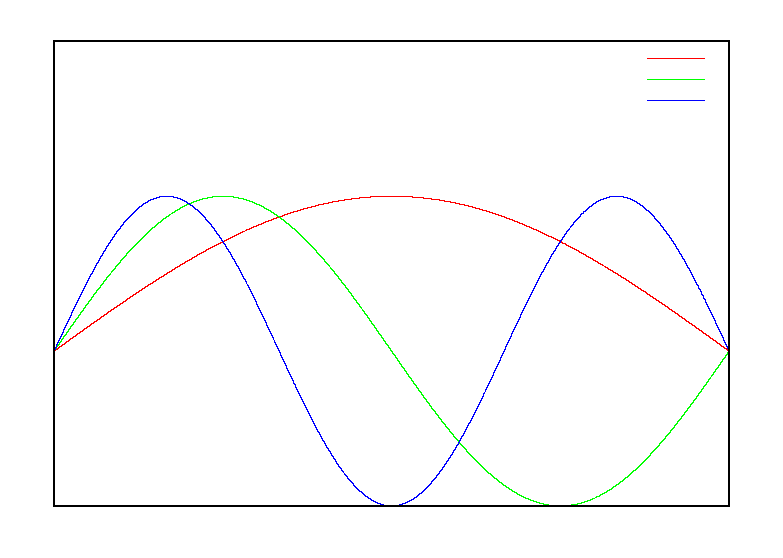
\includegraphics{TEM-moden}}%
    \gplfronttext
  \end{picture}%
\endgroup

	\caption[Räumliche Moden im Resonator]{Amplituden der
	fundamentalen Mode, der ersten und der zweiten Harmonischen in Abhängigkeit von einer
	räumlichen Dimension.}
	\label{fig:TEM-moden}
\end{figure}
Für TEM$_{mn,q}$ Moden ergeben sich die Frequenzen
\begin{equation}\label{eq:TEM-moden_frequenz}
	\nu_{mn,q}=\frac{c}{2d}\left[q+\frac{1}{2}(m+n+1)\right]\,.
\end{equation}
Im \textit{Single-Mode}-Laserbetrieb ist man bestrebt, nur die fundamentale Mode
TEM$_{00,q}$ zu erzeugen. Dies ist allerdings nur mit räumlich sehr eingeengten
Resonatoren möglich. Deshalb haben Single-Mode-Laserdioden eine aktive
Schicht mit einer Ausdehnung von $3\,$µm in lateraler und $1\,$µm in
transversaler Dimension und können nur begrenzte Ausgangsleistungen von bis zu
$150\,$mW erreichen. Höhere Ausgangsleistungen von bis zu $4\,$W sind nur mit
größeren aktiven Schichten von $50$ bis $400\,$µm in lateraler und $3\,$µm in transversaler Dimension
erreichbar.
Der sog. \textit{freie Spektralbereich} des Resonators ist der spektrale Abstand
von zwei möglichen Moden, die anschwingen können und ergibt sich für
TEM$_{00,q}$ Moden zu
\begin{equation}\label{eq:FSR_TEM-moden}
	\text{FSR}_{00,q}=\frac{c}{2d}\,.
\end{equation}
Da die typischen Werte des FSRs von infraroten Single-Mode-Laserdioden bei $150$
bis $600\,$GHz liegen und somit nur um ca. ein Zehntel kleiner sind als das
Verstärkungsprofil eines Diodenlasers in diesem Bereich ($30$ bis $50\,$nm), kann praktisch nur die fundamentale Mode anschwingen.

\subsubsection{Externer Resonator}\label{subsubsec:externer_resonator}
Die Frequenz eines Diodenlasers lässt sich durch Variation von Strom und
Temperatur verstimmen.
Ein höherer Strom führt zu einer stärkeren Besetzung des Valenzbandes und somit zu
einer kleineren effektiven Energielücke bzw. kleineren Frequenz. Gleichzeitig
wird allerdings durch Erhöhung des Brechungsindexes die Eigenfrequenz des
Resonators verringert. Selbstverständlich erhöht sich auch die Leistung des
Lasers. Eine Temperaturerhöhung bewirkt gleichermaßen eine stärkere Besetzung
des Valenzbandes und ebenfalls einen größeren Brechungsindex.\par
Da Strom und Temperatur jeweils auf zwei verschiedene Arten Einfluss auf die
Frequenz haben, müssten diese Parameter simultan variiert werden, was
allerdings enormen Einschränkungen unterliegt. Ein zu hoher Strom zerstört die
Diode. Zu niedrige Temperaturen führen zur Kondensation von Wasser an der Diode
und zu hohe Temperaturen zur Überhitzung. Zur größeren Verstimmbarkeit und wesentlich
höheren spektralen Selektivität werden deshalb externe Resonatoren eingesetzt.
Dabei verwendet man ein Gitter, dessen erste Ordnung wieder in die Diode
zurückgekoppelt wird. Die Rückkopplung führt zur Verstärkung des selektierten
Spektralbereichs. Die nullte Ordnung wird als Nutzstrahl ausgekoppelt. Dabei
gibt es zwei typische Aufbauten.\par
\begin{figure}[h]
 	\centering
 	\fbox{\parbox{\dimexpr \linewidth - 2\fboxrule - 2\fboxsep}{
		\subfloat[]{
			\label{subfig:externe_resonatoren_aufbau_littrow}
	    	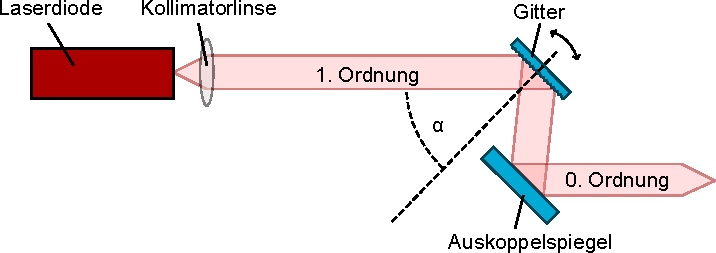
\includegraphics[width=\textwidth-1cm]{gfx/externe_resonatoren_aufbau_littrow}
	    	}\\
		\subfloat[]{
			\label{subfig:externe_resonatoren_aufbau_littmann}
	    	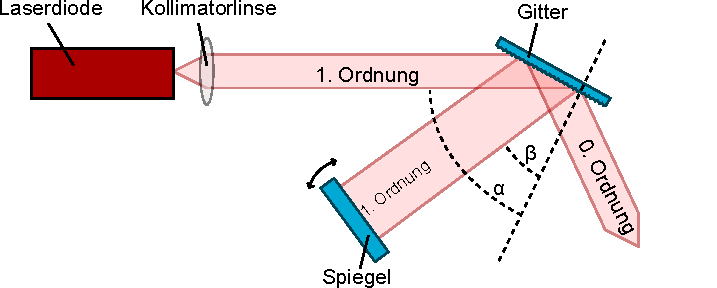
\includegraphics[width=\textwidth-1cm]{gfx/externe_resonatoren_aufbau_littmann}
	    	}
	}}
	\caption[Externe Resonatoren - Aufbau]{Externe
	Resonatoren im Littrow- (a) und im Littmann-Design
	(b).}
	\label{fig:externe_resonatoren_aufbau}
\end{figure}
Abbildung
\ref{fig:externe_resonatoren_aufbau}\subref{subfig:externe_resonatoren_aufbau_littrow} zeigt das sog.
\textit{Littrow-Design}, bei dem durch Verkippen des Gitters die Wellenlänge
\begin{equation}\label{eq:littrow}
	\lambda=2g\sin{(\alpha)}
\end{equation}
selektiert werden kann, wobei $g$ die Gitterkonstante ist. Durch Verdrehen eines
Auskoppelspiegels um dieselbe Achse kann die nullte Ordnung ohne Winkeländerung ausgekoppelt werden. Der
externe Resonator ist hierbei durch die hintere Wand der Diode und durch das
Gitter begrenzt.\par
Eine andere Variante ist das sog. \textit{Littman-Design} (siehe Abb.
\ref{fig:externe_resonatoren_aufbau}\subref{subfig:externe_resonatoren_aufbau_littmann}).
Dabei wird die erste Ordnung des Gitters auf einen Spiegel und auf demselben Weg wieder zurück in die
Diode gekoppelt. Die Wellenlänge
\begin{equation}\label{eq:littmann}
	\lambda=g\left[\sin{(\alpha)}+\sin{(\beta)}\right]
\end{equation}
ist nun vom Winkel des Spiegels abhängig. Durch die zweifache Frequenzselektion
am Gitter erreicht man wesentlich schmalere Linienbreiten, verliert jedoch
Leistung. Beim Verdrehen des Gitter im Littrow-Design bzw. des Spiegel im
Littmann-Design muss darauf geachtet werden, dass ebenfalls die Resonatorlänge
angepasst wird. Dies kann durch eine geschickt gewählte Drehachse realisiert
werden.\par Die anschwingende Mode kombiniert sich nun aus internem und externem Modenprofil
wie in Abb. \ref{fig:moden_frequenzselektion} dargestellt.
\begin{figure}[h]
	\footnotesize	
	\centering
	\subfloat[]{
		\label{subfig:moden_frequenzselektion_a}
		% GNUPLOT: LaTeX picture with Postscript
\begingroup
  \makeatletter
  \providecommand\color[2][]{%
    \GenericError{(gnuplot) \space\space\space\@spaces}{%
      Package color not loaded in conjunction with
      terminal option `colourtext'%
    }{See the gnuplot documentation for explanation.%
    }{Either use 'blacktext' in gnuplot or load the package
      color.sty in LaTeX.}%
    \renewcommand\color[2][]{}%
  }%
  \providecommand\includegraphics[2][]{%
    \GenericError{(gnuplot) \space\space\space\@spaces}{%
      Package graphicx or graphics not loaded%
    }{See the gnuplot documentation for explanation.%
    }{The gnuplot epslatex terminal needs graphicx.sty or graphics.sty.}%
    \renewcommand\includegraphics[2][]{}%
  }%
  \providecommand\rotatebox[2]{#2}%
  \@ifundefined{ifGPcolor}{%
    \newif\ifGPcolor
    \GPcolortrue
  }{}%
  \@ifundefined{ifGPblacktext}{%
    \newif\ifGPblacktext
    \GPblacktexttrue
  }{}%
  % define a \g@addto@macro without @ in the name:
  \let\gplgaddtomacro\g@addto@macro
  % define empty templates for all commands taking text:
  \gdef\gplbacktext{}%
  \gdef\gplfronttext{}%
  \makeatother
  \ifGPblacktext
    % no textcolor at all
    \def\colorrgb#1{}%
    \def\colorgray#1{}%
  \else
    % gray or color?
    \ifGPcolor
      \def\colorrgb#1{\color[rgb]{#1}}%
      \def\colorgray#1{\color[gray]{#1}}%
      \expandafter\def\csname LTw\endcsname{\color{white}}%
      \expandafter\def\csname LTb\endcsname{\color{black}}%
      \expandafter\def\csname LTa\endcsname{\color{black}}%
      \expandafter\def\csname LT0\endcsname{\color[rgb]{1,0,0}}%
      \expandafter\def\csname LT1\endcsname{\color[rgb]{0,1,0}}%
      \expandafter\def\csname LT2\endcsname{\color[rgb]{0,0,1}}%
      \expandafter\def\csname LT3\endcsname{\color[rgb]{1,0,1}}%
      \expandafter\def\csname LT4\endcsname{\color[rgb]{0,1,1}}%
      \expandafter\def\csname LT5\endcsname{\color[rgb]{1,1,0}}%
      \expandafter\def\csname LT6\endcsname{\color[rgb]{0,0,0}}%
      \expandafter\def\csname LT7\endcsname{\color[rgb]{1,0.3,0}}%
      \expandafter\def\csname LT8\endcsname{\color[rgb]{0.5,0.5,0.5}}%
    \else
      % gray
      \def\colorrgb#1{\color{black}}%
      \def\colorgray#1{\color[gray]{#1}}%
      \expandafter\def\csname LTw\endcsname{\color{white}}%
      \expandafter\def\csname LTb\endcsname{\color{black}}%
      \expandafter\def\csname LTa\endcsname{\color{black}}%
      \expandafter\def\csname LT0\endcsname{\color{black}}%
      \expandafter\def\csname LT1\endcsname{\color{black}}%
      \expandafter\def\csname LT2\endcsname{\color{black}}%
      \expandafter\def\csname LT3\endcsname{\color{black}}%
      \expandafter\def\csname LT4\endcsname{\color{black}}%
      \expandafter\def\csname LT5\endcsname{\color{black}}%
      \expandafter\def\csname LT6\endcsname{\color{black}}%
      \expandafter\def\csname LT7\endcsname{\color{black}}%
      \expandafter\def\csname LT8\endcsname{\color{black}}%
    \fi
  \fi
  \setlength{\unitlength}{0.0500bp}%
  \begin{picture}(7200.00,5040.00)%
    \gplgaddtomacro\gplbacktext{%
      \csname LTb\endcsname%
      \put(160,2569){\rotatebox{-270}{\makebox(0,0){\strut{}Verst{"a}rkung}}}%
      \put(3599,140){\makebox(0,0){\strut{}Frequenz}}%
      \put(1440,3640){\makebox(0,0)[l]{\strut{}anschwingende Mode}}%
    }%
    \gplgaddtomacro\gplfronttext{%
      \csname LTb\endcsname%
      \put(5936,4636){\makebox(0,0)[r]{\strut{}Verst{"a}rkungs-Profil}}%
      \csname LTb\endcsname%
      \put(5936,4436){\makebox(0,0)[r]{\strut{}interne Moden}}%
      \csname LTb\endcsname%
      \put(5936,4236){\makebox(0,0)[r]{\strut{}Winkeldispersion des Gitters}}%
      \csname LTb\endcsname%
      \put(5936,4036){\makebox(0,0)[r]{\strut{}externe Moden}}%
      \csname LTb\endcsname%
      \put(5936,3836){\makebox(0,0)[r]{\strut{}gesamte Verst{"a}rkung}}%
    }%
    \gplbacktext
    \put(0,0){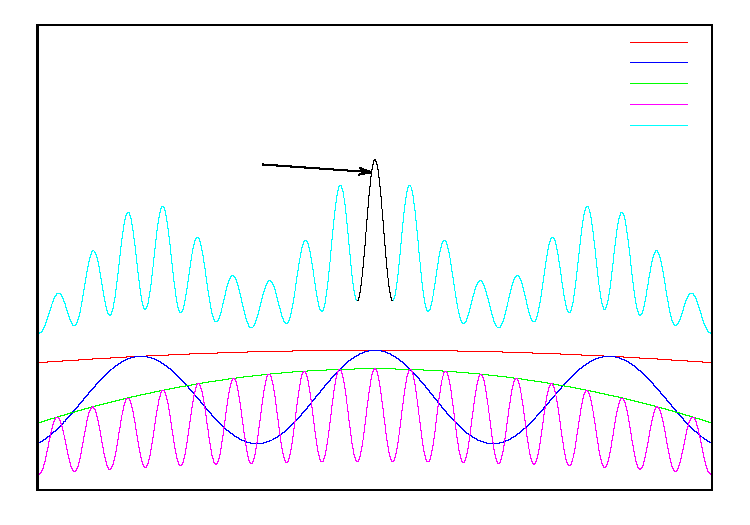
\includegraphics{moden_frequenzselektion_a}}%
    \gplfronttext
  \end{picture}%
\endgroup

  	}\\
	\subfloat[]{
		\label{subfig:moden_frequenzselektion_b}
		% GNUPLOT: LaTeX picture with Postscript
\begingroup
  \makeatletter
  \providecommand\color[2][]{%
    \GenericError{(gnuplot) \space\space\space\@spaces}{%
      Package color not loaded in conjunction with
      terminal option `colourtext'%
    }{See the gnuplot documentation for explanation.%
    }{Either use 'blacktext' in gnuplot or load the package
      color.sty in LaTeX.}%
    \renewcommand\color[2][]{}%
  }%
  \providecommand\includegraphics[2][]{%
    \GenericError{(gnuplot) \space\space\space\@spaces}{%
      Package graphicx or graphics not loaded%
    }{See the gnuplot documentation for explanation.%
    }{The gnuplot epslatex terminal needs graphicx.sty or graphics.sty.}%
    \renewcommand\includegraphics[2][]{}%
  }%
  \providecommand\rotatebox[2]{#2}%
  \@ifundefined{ifGPcolor}{%
    \newif\ifGPcolor
    \GPcolortrue
  }{}%
  \@ifundefined{ifGPblacktext}{%
    \newif\ifGPblacktext
    \GPblacktexttrue
  }{}%
  % define a \g@addto@macro without @ in the name:
  \let\gplgaddtomacro\g@addto@macro
  % define empty templates for all commands taking text:
  \gdef\gplbacktext{}%
  \gdef\gplfronttext{}%
  \makeatother
  \ifGPblacktext
    % no textcolor at all
    \def\colorrgb#1{}%
    \def\colorgray#1{}%
  \else
    % gray or color?
    \ifGPcolor
      \def\colorrgb#1{\color[rgb]{#1}}%
      \def\colorgray#1{\color[gray]{#1}}%
      \expandafter\def\csname LTw\endcsname{\color{white}}%
      \expandafter\def\csname LTb\endcsname{\color{black}}%
      \expandafter\def\csname LTa\endcsname{\color{black}}%
      \expandafter\def\csname LT0\endcsname{\color[rgb]{1,0,0}}%
      \expandafter\def\csname LT1\endcsname{\color[rgb]{0,1,0}}%
      \expandafter\def\csname LT2\endcsname{\color[rgb]{0,0,1}}%
      \expandafter\def\csname LT3\endcsname{\color[rgb]{1,0,1}}%
      \expandafter\def\csname LT4\endcsname{\color[rgb]{0,1,1}}%
      \expandafter\def\csname LT5\endcsname{\color[rgb]{1,1,0}}%
      \expandafter\def\csname LT6\endcsname{\color[rgb]{0,0,0}}%
      \expandafter\def\csname LT7\endcsname{\color[rgb]{1,0.3,0}}%
      \expandafter\def\csname LT8\endcsname{\color[rgb]{0.5,0.5,0.5}}%
    \else
      % gray
      \def\colorrgb#1{\color{black}}%
      \def\colorgray#1{\color[gray]{#1}}%
      \expandafter\def\csname LTw\endcsname{\color{white}}%
      \expandafter\def\csname LTb\endcsname{\color{black}}%
      \expandafter\def\csname LTa\endcsname{\color{black}}%
      \expandafter\def\csname LT0\endcsname{\color{black}}%
      \expandafter\def\csname LT1\endcsname{\color{black}}%
      \expandafter\def\csname LT2\endcsname{\color{black}}%
      \expandafter\def\csname LT3\endcsname{\color{black}}%
      \expandafter\def\csname LT4\endcsname{\color{black}}%
      \expandafter\def\csname LT5\endcsname{\color{black}}%
      \expandafter\def\csname LT6\endcsname{\color{black}}%
      \expandafter\def\csname LT7\endcsname{\color{black}}%
      \expandafter\def\csname LT8\endcsname{\color{black}}%
    \fi
  \fi
  \setlength{\unitlength}{0.0500bp}%
  \begin{picture}(7200.00,5040.00)%
    \gplgaddtomacro\gplbacktext{%
      \csname LTb\endcsname%
      \put(160,2569){\rotatebox{-270}{\makebox(0,0){\strut{}Verst{"a}rkung}}}%
      \put(3599,140){\makebox(0,0){\strut{}Frequenz}}%
      \put(900,3729){\makebox(0,0)[l]{\strut{}Modensprung bzw. Multi-Mode}}%
    }%
    \gplgaddtomacro\gplfronttext{%
      \csname LTb\endcsname%
      \put(5936,4636){\makebox(0,0)[r]{\strut{}Verst{"a}rkungs-Profil}}%
      \csname LTb\endcsname%
      \put(5936,4436){\makebox(0,0)[r]{\strut{}interne Moden}}%
      \csname LTb\endcsname%
      \put(5936,4236){\makebox(0,0)[r]{\strut{}Winkeldispersion des Gitters}}%
      \csname LTb\endcsname%
      \put(5936,4036){\makebox(0,0)[r]{\strut{}externe Moden}}%
      \csname LTb\endcsname%
      \put(5936,3836){\makebox(0,0)[r]{\strut{}gesamte Verst{"a}rkung}}%
    }%
    \gplbacktext
    \put(0,0){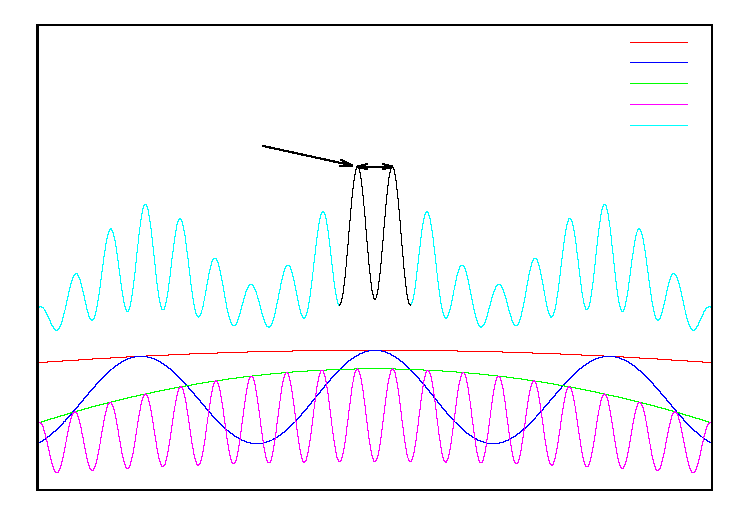
\includegraphics{moden_frequenzselektion_b}}%
    \gplfronttext
  \end{picture}%
\endgroup

  	}
	\caption[Diodenlaser - Verstärkungsprofil]{Verstärkungsprofil, internes und
	externes Modenprofil und anschwingende Mode des Lasers. (a) zeigt eine
	Konfiguration, bei der eine einzige Mode anschwingt.
	(b) zeigt den Grenzfall, bei dem zwei Moden anschwingen können. $\rightarrow$
	Modensprung bzw. Multi-Mode}
	\label{fig:moden_frequenzselektion}
\end{figure}
Nur die Mode mit der größten Verstärkung schwingt an, alle anderen
werden unterdrückt, wie in Abb.
\ref{fig:moden_frequenzselektion}\subref{subfig:moden_frequenzselektion_a} zu sehen ist.
Damit die Frequenz über einen möglichst großen Bereich verstimmt werden kann,
muss das Modenprofil des internen und externen Resonators gleichzeitig verstimmt
werden. Strom und Gitterwinkel müssen also simultan verstimmt werden, wobei das
Gitter mithilfe eines Piezoaktuators verdreht werden kann. Dieses Verfahren
nennt man \textit{Feed Forward}. Verstimmt man nur einen Resonator oder verstimmt
man beide Resonatoren in falscher Relation kommt es zu
\textit{Modensprüngen}, wie
\ref{fig:moden_frequenzselektion}\subref{subfig:moden_frequenzselektion_a} zeigt.\par Alternativ ist es auch möglich ein \textit{Antireflex-coating (AR-coating)} für
die Diode zu verwenden, und somit den Laser ohne internen Resonator zu
betreiben.
Dies bringt den Vorteil, dass nur noch der Gitterwinkel verstellt werden muss
und der Strom und somit auch weitestgehend die Leistung konstant bleiben.
Nachteil ist, dass die Diode alleine nicht mehr als Laserdiode verwendet werden kann, da
der notwendige Resonator fehlt.

\subsubsection{Leistung}\label{subsubsec:diodenlaser_leistung}
Für den autoionisierenden Schritt in der RIS werden gewöhnlich sehr viel höhere
Leistungen ($>200\,$mW) benötigt als mit Single-Mode-Dioden möglich ist. Mit
einem \textit{Trapezverstärker} können im roten Bereich durch
\textit{Injection-Seeding} Leistungen von über $1\,$W erreicht werden. Nähere
Erklärungen finden sich in \cite{schumann:2001:diplomarbeit}.